% document definition 
\documentclass[a4paper,11pt]{article} 

% create the following file in the input from the template
\newcommand{\PaperTitle} {Report on Research and Development}
\newcommand{\PaperSubject} {\textbf{Use of Recommender System in Robotics}}
\newcommand{\PaperDate} {\today}
\newcommand{\PaperLecturer} {Prof. Dr. Paul Pl{\"o}ger and M.Sc. Iman Awaad}
\newcommand{\PaperLecturerEMail} {mailto:paul.ploeger@h-brs.de, iman.awaad@h-brs.de}
\newcommand{\Paperkeywords} {Recommender System, Programming by Demonstration, robotic skills, industrial robots}
\newcommand{\PaperMainWriter} {Deebul Nair}
\newcommand{\PaperMainWriterEMail} {mailto:deebul.nair@smail.inf.fh-bonn-rhein-sieg.de}

\usepackage[latin1]{inputenc} 
\usepackage{graphics}
\usepackage{url}

\usepackage{mya4page}
\usepackage{amsmath}
\usepackage[hidelinks=true]{hyperref}
\usepackage{bibnames}
\usepackage{path}
\usepackage{setspace}
\usepackage{epsfig}
\usepackage{multirow}
\usepackage[]{algorithm2e}
\usepackage[acronym]{glossaries}
\usepackage{graphicx}
\usepackage{caption}
\usepackage{subcaption}
\usepackage{placeins}
%\usepackage{footmisc}
%\usepackage[perpage,symbol*]{footmisc} 

%---------------------------------------------------------------
\usepackage{color}
%% Hyperref setup
\usepackage{hyperref}
\hypersetup{
   pdftitle={ \PaperTitle },
   pdfsubject={ \PaperSubject },
   pdfauthor={ \PaperMainWriter <deebul.nair@smail.inf.fh-bonn-rhein-sieg.de>},
   pdfkeywords={ \Paperkeywords },
   bookmarksopen=true
}

%\newcommand{\picHere}[3] { %
\begin{figure}[htp] %
\begin{center} %
\resizebox{!}{!}{\includegraphics{pictures/#1}} %
\caption{{\small#2}} %
\label{#3} %
\end{center} %
\end{figure} %
}

\newcommand{\picHereWidth}[4] { %
\begin{figure}[htp] %
\begin{center} %
\resizebox{!}{!}{\includegraphics[#4]{pictures/#1}} %
\caption{{\small#2}} %
\label{#3} %
\end{center} %
\end{figure} %
}

\newcommand{\picHereRes}[3] { %
\begin{figure}[htp] %
\begin{center} %
\resizebox{!}{!}{\includegraphics[totalheight=0.8\textheight]{pictures/#1}} %
\caption{#2} %
\label{#3} %
\end{center} % 
\end{figure} %
}

\makeglossaries
 
\newacronym{lfd}{LfD}{Learning from Demonstration}
\newacronym{mp}{MP's}{Motion primitives}
\newacronym{hmm}{HMM}{Hidden Markov Model}
\newacronym{gmm}{GMM}{Gaussian Mixture Model}
\newacronym{tec}{TEC}{Theory of event coding}
\newacronym{hmi}{HMI}{Human Machine Interaction}
\newacronym{ndcg}{nDCG}{normalized discounted cumulative gain}

\begin{document}
\singlespacing
\pagenumbering{roman}
% create title template 
\title{\PaperTitle\\\PaperSubject}
\author{\href{\PaperMainWriterEMail}{\PaperMainWriter \footnote{\href{\PaperMainWriterEMail} {deebul.nair@smail.inf.fh-bonn-rhein-sieg.de}} 
}\\%\vspace{0.5cm} \\ 
Matrikel Nr.: 9023573 \vspace{0.5cm} \\ 
B-IT Master Studies Autonomous Systems \vspace{0.5cm} \\ 
University of Applied Sciences Bonn-Rhein-Sieg\\ % \vspace{0.1cm}
Fraunhofer Institute for Autonomous Intelligent Systems \vspace{0.7cm} \\ \setcounter{footnote}{6}
Advisor: \PaperLecturer  
}%\small{\PaperTerm}}
%\date{April 29, 2003}%\PaperDate}
%\date{July 11, 2003}
\maketitle

\onehalfspacing
\newpage
% crate abstract template 
\begin{abstract}
   Learning from Demonstration covers methods by which a robot learns new skills
   using human guidance. Learning from Demonstration in robotic systems involves a
   number of important aspects, such as deducing the relevant features of the
   observations, modelling  based on the relevant features and execution
   based on the model. We consider the problem of inferring the pertinent
   features using a set of demonstrations, that should be reproduced by the
   robot. This is challenging because the number of demonstrations on which the
   learning has to be made are few. In this work, we improvise an approach which
   is inspired by recommender systems to have an expert knowledge base. This
   knowledge base is then used to recommend the relevant features to imitate .
   The expert knowledge base is a reduced subset of the whole search space of
   the features to be imitated. The key novelty  of our work is in the expert
   knowledge base used for recommendation, which is structured based on effect
   metrics. We argue that the structured knowledge base helps in inferring the
   relevant features using very less demonstrations. In this work we use the
   skill based framework for robot programming. Under this framework we try to
   learn the \textif{"move"} motion primitive. The relevant features for successful
   reproduction of the \textif{"move"} motion primitive are learnt using the method
   proposed. The approach was evaluated in simulation and using data acquired
   from the youBot robot. The results shows promising progress as it could
   learn with less number of demonstrations.
\end{abstract}


\newpage
\tableofcontents
\newpage
\listoffigures
 \newpage
\listoftables

\newpage
 
\printglossary[type=\acronymtype, title=Acronyms]
\clearpage
\pagenumbering{arabic}
% document content begin here
\section{Introduction} 
\acrfull{lfd} is a technique of learning new skills based on
demonstrations by a teacher\cite{argall_survey_2009}. In 2013, robot sales
increased by 12 \% to 178,132 units, by far the highest level ever recorded for
one year. Sales of industrial robots to the automotive, the chemical, and the
rubber and plastics industries, as well as to the food industry continued to
increase in 2013. Between 2008 and 2013 the average robot sales increase was at
9.5\% compounded annual growth rate per year
\footnote{\url{http://www.ifr.org/uploads/media/Executive_Summary_WR_2014_02.pdf
}}. With the increasing number of robots being deployed in the industries the
amount of efforts to program the robots is also increasing. It is a major
requirement to program the robots with new tasks even by persons who are non
experts in robotics. \acrshort{lfd} comes as an appropriate solution to this problem, in
which a non expert can demonstrate the expected skill to the robot and the
robot can learn from it.


In our work we work on the problem of inferring the relevant aspects of the
demonstration for a successful reproduction of a motion primitive. A motion
primitive is defined as a single elementary movement
\cite{schaal_nonlinear_2000}. Motion primitive forms the building blocks for
the robotic skills, which in turn forms building blocks of robotic tasks. For
example we want the robot to do a task \textit{"Get milk bottle from the
refrigerator."}. This task can be broken down into various robotic skills
\textit{moveto(refrigerator) + open(refrigerator) + pickup(milk bottle) +
close(refrigerator) + moveto(table)}. Each of the robotic skills can be
composed of several atomic movements i.e. motion primitives . So the skill of
\textit{pickup} can be composed of \textit{$move\_arm$(milk bottle) + grasp(milk
bottle) + $move\_arm$(tray) + release(milk bottle)} motion primitives. Thus each
task of the robot can be broken down to the level of atomic actions of the
motion primitives. The motion primitives are executed in a sequence to achieve
the higher goals.

Motion primitives in robotics is a highly researched topic. There are various
representation of motion primitives available in the literature. In our
approach we propose a feature based representation for the motion primitive. A
feature is a quantitative element of the world the robot can measure. In our
approach we identify the relevant features that completely describe a motion
primitive. The general approach taken in machine learning for the problem is to
create a large training dataset and use feature selection algorithms to
determine the relevant features. But this approach cannot be used in \acrshort{lfd} since
the demonstrations which are the training dataset, are sparse.


In \cite{abdo_inferring_2014} came up with a novel idea for determining
relevant features using few demonstrations by taking inspirations from
recommender systems . They build an off-line expert knowledge base using
experts, which is similar to the user preferences created by recommender
system. Now the expert knowledge base is used to make a recommendations on the
relevant features of the motion primitive.


Our work advances the approach of \cite{abdo_inferring_2014}, such that the
knowledge base created is more structured using effect metrics. Effect metrics
are a means of measuring changes which have occurred in the robot, environment
and interactions of robot-environment due to an action.  The knowledge base is
collected off-line and before any demonstrations. When a new motion primitive
is learned, the demonstrations are shown by an user. The robot, based on the
data available from demonstrations and the off-line knowledge base makes
recommendations on what are the relevant features for the motion primitive.


\subsection{Why not the term "recommender system" ?}
The work should be ideally named as "Learning by Demonstration, recommendation
using Expert knowledge base". The name "recommender system" is an established
term in literature. Recommender systems are a subclass of information filtering
systems that seek to predict the 'rating' or 'preference' that a user would
give to an item \cite{bobadilla_recommender_2013}. The prediction of the
preference is done based on a knowledge base generated using the user data.
This knowledge base generation is always an online process. But in our work we
try to create the knowledge base off-line that is based on expert knowledge.
Also in our case the system recommends set of features that could be used to
explain a demonstrated motion primitive by doing a greedy search on all the
templates available in the knowledge base. This is not the case in recommender
systems. So even though in principle the idea of both the systems are same, we
would like to refrain from using the term recommender system and rather use a
more generic term "recommendations using knowledge base".

\newpage
\section{Problem Statement}

\acrfull{lfd} is defined as a technique that develops policy from examining
state to action mappings \cite{argall_survey_2009}. The state are expressed in
terms of the features and the actions are the motion primitives. The action
causes changes in the state of the world. The world consist of the robot and
the environment. 

The \acrshort{lfd} problem can be defined as follows \cite{argall_survey_2009}. 

The world consist of states $S$ and actions $A$. The mapping between states by
way of actions is defined by a probabilistic transition function $T(s`|s, a) $
; $S \times A \times S \rightarrow [0,1]$. $s`$ is the resultant state due to
the execution of the action $a$ on the initial state $s$. As we all know the
world is not fully observable all the time. Only a part of the world $Z$ is
observable. The learning has to be made on the observable states $Z$.

A policy $\pi : Z \rightarrow A $ selects action based on observations of world
state. A policy determines which action $a$ to execute from $A$ based on the
observations $Z$. 


The demonstrations used in our approach consist of pairs of initial state and
final state. Initial state is the state before the execution of an action while
final state is the state after the execution of the state. The demonstrations
$d$ consist of pairs of demonstrated initial state $z$ and final state $z`$
Demonstrations $d \in D$ formally as $k$ pairs of initial-final states: $d =
{(z^i , {z`}^i)} \text{where} (z^i, {z`}^i) \in Z \text{and}  i = 0,...,k$

\subsection{Deriving a policy: Goal based mapping}

In these methods of policy learning of \acrshort{lfd}, the policy tries to
predict the state of the world once the action is executed based on the current
state of the world.

The perspective adopted is that multiple demonstrations of the same action can
help to understand the key aspects of the action. In other words, when an
action shares similar goal across multiple demonstrations, it might suggest
that corresponding goal must be achieved in-order to reproduce the action. So
these methods of policy learning takes the demonstrations as input and provides
a list of goals to be satisfied as output for reproduction of the action.

This prediction is the passed to a planner who tries to find a plan to execute
the action to reach the predicted goal state as illustrated in figure \ref{goal
based learning}(\cite{argall_survey_2009})
\begin{figure}[htp]
\centering
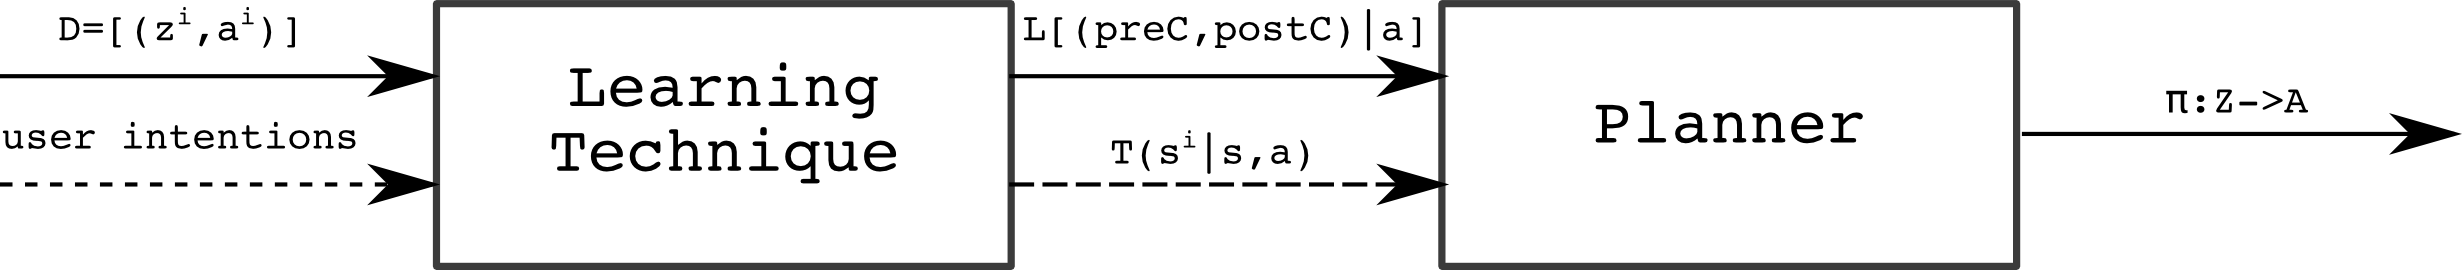
\includegraphics[scale=0.8]{images/plans_policy_derivation.png}
\caption[Deriving a policy : goal based]{Policy Derivation by determining the
goal of the actions \cite{argall_survey_2009}}
\label{goal based learning}
\end{figure}
\subsection {Goal based mapping on relevant features}

The policy learning with the complete set of features of the observed states
faces a drawback that it requires a lot of demonstrations. So to learn on fewer
demonstrations we need to do determine the relevant features of the states and
do the policy learning only based on these relevant features.

When an action shares similar components across multiple demonstrations, it
might suggest that these components are the essential features of the state
that should be reproduced by the robot. In these methods the relevant features
$R$ of the states are determined based on the likelihoods of the
demonstrations, before the goal state prediction.

The policy learning technique first determines which are the relevant aspects
of the states for reproducing the action and these are then provided to the
predictor function which predicts the goal state as illustrated in figure
\ref{feature goal based learning} (modified from \cite{argall_survey_2009}) .

\begin{figure}[htp]
\centering
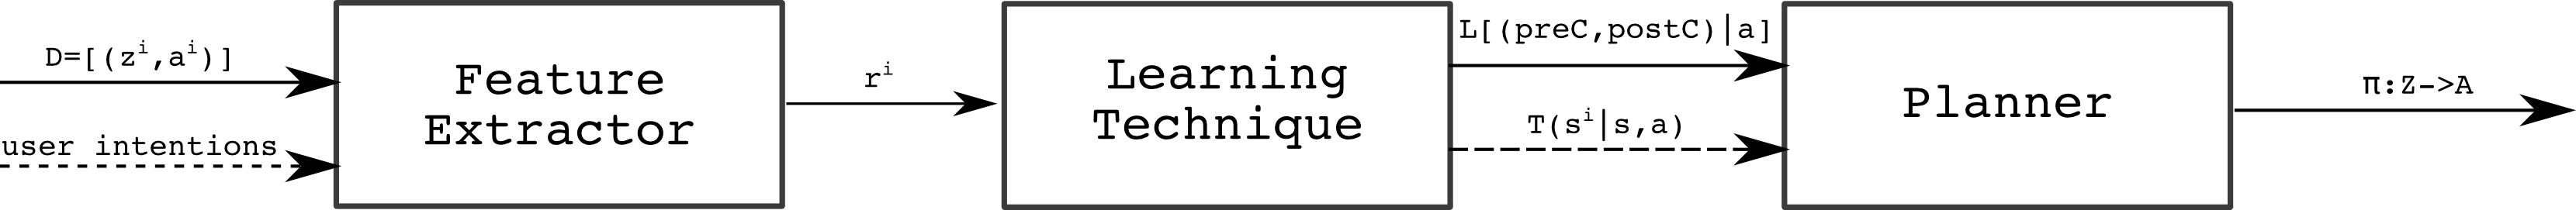
\includegraphics[scale=0.6]{images/features_plans_policy_derivation.png}
\caption[Deriving a policy : feature based ]{Policy derivation using first
extracting relevant features and then determining the goal state of the robot
(modified from \cite{argall_survey_2009})}
\label{feature goal based learning}
\end{figure}


\newpage
\section{ Related Work } 
\subsection{Motion Primitives}

Motion primitives is a well defined concept for representing modular and
re-usable skills in robotics. Motion primitive can be considered as
elementary building blocks for skill representation \cite{kruger_learning_2010}.
Motion primitives are commonly used for representing and learning skills in
robotics.

There is generally two distinct approaches to represent motion primitives, one
at the trajectory level and the other at the symbolic level \cite{argall_survey_2009}.
One of the early techniques in the trajectory level approaches was as a spline
by \cite{ude_trajectory_1993}. The other most common method is to represent
motion primitives as a  probabilistic representation \cite{calinon_robot_2009}.
\acrfull{gmm} is used to encode motion primitives through probabilistic
representation. \acrshort{gmm} allowed autonomous and incremental construction
of the motion primitives. This was beneficial for \acrshort{lfd}. \acrfull{hmm}
is used to encode motion primitives. In \acrshort{hmm} the motion primitives
are represented as a single multivariate Gaussian Distribution.
\cite{paraschos_probabilistic_2013} introduced the concept of probabilistic
movement primitives (Promotion primitives) as generalistic framework for
representing and learning motion primitives.

A popular alternative to this approach has considered modelling the intrinsic
dynamics of motion \cite{schaal_nonlinear_2000} . This approach was advantageous
for \acrshort{lfd} as it was time-independent and can be modulated to produce trajectories
with similar dynamics in area of workspace not covered during learning. One of
the drawbacks of the trajectory based techniques was that it lacks cognitive
sense \cite{aein_toward_2013}. These
drawbacks are also been addressed in current research activities like
\cite{manschitz_learning_2015} where the transition between
the motion primitives are also being learned to execute complex tasks.

In symbolic representations a compact descriptions of motion primitives is defined, but the
execution details are not included. A large body of work uses symbolic
representation for encoding motion primitives (\cite{muench_robot_1994},
\cite{friedrich_robot_1996}, \cite{pardowitz_incremental_2007}).
\cite{alissandrakis_approach_2005} encoded human motions as
pre-defined postures, positions or configurations. \cite{aein_toward_2013} creates a library
of motion primitives. In a more recent work by \cite{andersen_using_2014} the skill
based framework is used to learn predefined
skills. The skills are made of combinations of motion primitives. The configuration
parameters of the motion primitives are learnt by demonstrations. The paper proposes an
approach to represent skill for learning inside a skill based framework.
But in the above work the representation of motion primitives in a skill based framework is
not well defined.

\subsubsection{Proposed Motion Primitive }
\label{sec:Proposed motion primitive}
We represent motion primitives as foundation blocks
for a robot to complete a skill. For example consider a "pick up skill" can be
executed using combinations of "move" Motion primitive. So a \textit{pick up screw}
skill gets fragmented as \textit{move arm camera pose} + \textit{move arm grasp pose} + \textit{move
arm place pose}. Which motion primitives are available to a robot depends on the hardware
specification of the robot.

Each motion primitives has a pre-condition and post-conditions to ensure and verify a proper
functioning. Using \acrshort{lfd} we try to learn the post-condition(goal) of the motion primitives. The
motion primitives in our framework consist of a teaching part and an execution phase, as
illustrated in Figure \ref{motion primitive} (extended from \cite{bogh_does_2012} and \cite{andersen_using_2014})
The motion primitive using this approach is well suited for the skill
based framework as explained in \cite{pedersen_robot_2015}. 
\begin{figure}[htp] \centering
    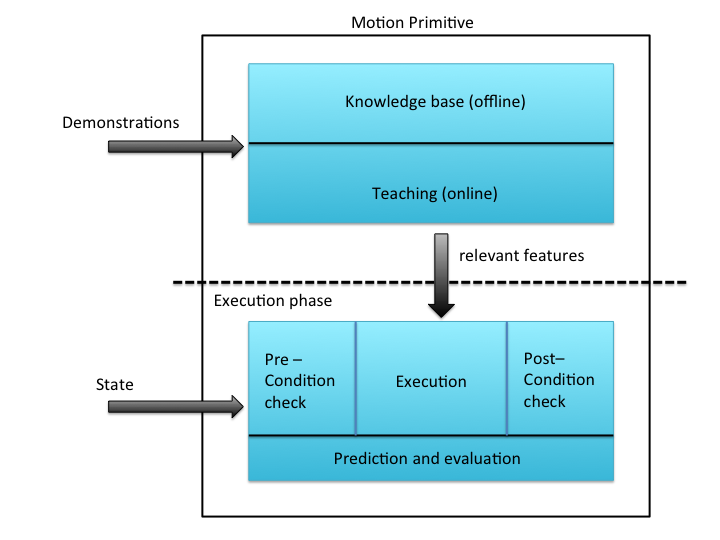
\includegraphics[scale=0.5]{images/motion_primitive_color.png}
    \caption[General structure of a motion primitive]{Proposed general
    structure of a motion primitive. A motion primitive consist of Learning
Phase and Execution Phase.} \label{motion primitive} \end{figure}

The motion primitive as shown in figure \ref{motion primitive} consist of two parts 
the learning part and the execution part.
In the learning part the demonstrations are taken as an input and the relevant features are 
extracted. This extracted features are then fed to the execution part.
The execution part is represented as a combination of pre and post conditions of features.
Based on the relevant features the execution phase predicts the post conditions 
and executes  the motion primitive.
In section \ref{sec:Learning motion primitive} the mathematical formulation of the 
motion primitive is discussed in details.

\subsection{Goal Based Learning from Demonstration}
A large body of work uses
goal based or plan based representation of learning\\
(\cite{friedrich_robot_1995},
\cite{nicolescu_natural_2003}, \cite{csibra_obsessed_2007}, \cite{demiris_prediction_2007},
\cite{veeraraghavan_teaching_2008}, \cite{lee_effective_2009}, \cite{hommel_action_2009}, \\ 
\cite{abdo_learning_2013}). 
The majority of the work in these try to infer the underlying goals and intent of
the demonstrator. The terms goals and intent are used interchangeable; but
goal refers to the immediate desirable state while intent refers to longer term
desirable state. \cite{tomasello_understanding_2005} defines intent as \textit{" a plan of
    action the organisam chooses and commits itself to the pursuit of a goal,
an intention thus includes both a means(action plan) as well as goal"}(p676).

The idea of learning goals is inspired by learning techniques in humans. It has
been studies that humans show a strong and early indication to interpret
observed behaviours of others as goal directed actions. This is termed as
'teleological obsession' \cite{ csibra_obsessed_2007} . They argue this
'teleological obsession' serves for on-line prediction and social learning.

The problem of recognizing goals and intentions of the action can be formulated
as a problem of model matching. The agent which is observing deploys sensors,
each reporting its observations of the state. Based on the state observations, two
approaches are available for analysis \textit{descriptive} and \textit{generative}
\cite { demiris_prediction_2007}

In \textit{generative} approach the observed states are mapped into a latent(hidden)
space. The latent space is usually of lower dimension than the observation
space. The main problem of inferring in the observation space is the
dimensionality of the space. So by reducing the observations to latent space
learning is made on smaller dimensions. Generative model is highly popular in
machine learning community and robotics community (\cite{buxton_learning_2003}, \cite{bishop_pattern_2006}
, \cite{calinon_robot_2009})

In contrast, in the  \textit{descriptive} approach, the patterns are characterised by
extraction of a number of low level features, and to use the set of
restrictions of the features level(\cite{isham_introduction_1981}, \cite{jain_deformable_1998}, 
\cite{abdo_learning_2013}). The
observer agent subsequently matches the observed data against pre-existing
representations and depending on what the task is show generates the action
corresponding to their representations. Pre -existing representations can have
associated data that label these representations with the goals, beliefs and
intentions that underlie in the demonstrations. This approach corresponds to the \acrfull{tec}
method for intention interpretation by \cite{csibra_obsessed_2007}. \acrshort{tec} was formulated
to provide an alternative prespective that allows to take intentions and the
goal directed nature of action into consideration. \acrshort{tec} explains how human
learning works; basically how human action is anticipatory in nature, how
anticipation emerge from experience and, how anticipation comes to regulate
human behaviour.

Our work is an extension of the \textit{descriptive} approach of learning. We also learn
using the restircted feature space.

\subsubsection{Proposed Expert Knowledge Base} 
A recent work by \cite{abdo_inferring_2014} leverages feedback from experts to create a
recommendations and use this recommendations to recommend features for actions.
Our approach advances over \cite{abdo_inferring_2014}, by creating  a more structured
knowledge base . The expert knowledge base used in the previous is not
structured. In this work we try to create a more structured generic framework
based on effect metrics concept. The expert knowledge base is explained in 
details in the section \ref{sec:Learning motion primitive}.

\subsection{Recommender system in Robotics}
Use of the recommender system in robotics is a very recent affair. Recommender
system is a special branch in machine learning which specializes in determining
the user preferences, based on previous activites of the user. It then uses
this user preferences to predict products(movies, videos, news etc) which the
user will like to see or purchase. Recommender systems are broadly classified
into two types \textit{Content Based Recommender System} and
\textit{Collabrative Recommender System} \cite{bobadilla_recommender_2013}. The use of recommender system in
robotics is relative a new approach. The first to use was by \cite{matikainen_model_2012},
who used it to the model recommendation problem. They tried to recommend based
on previous history which machine learning algorithm to use for a specific
image processing situation. In \cite{matikainen_multi-armed_2013} they tried to
solve the n-bandit problem of selecting food floor coverage statistics using
recommender system.

Further Recommender system was used to learn user preferences of the users for
doing daily chorus for robots. \cite{abdo_collaborative_2014} and
\cite{abdo_robot_2015} tried to learn user preferences concerning a given
tasks using small number of known preferences. Using recommender system they
enable robots to predict user preferences with respect to tidying up objects in
containers,  such  as  shelves  or  boxes.




\newpage
\section{Learning Motion Primitive using Kinesthetic Demonstrations}
\label{sec:Learning motion primitive}
The main idea of the work is to infer the relevant set of features,
which describe the demonstrated motion primitive.
Based on the learnt relevant features, during the execution phase 
the robot tries to predict the goal of the motion primitive, starting 
from a new initial condition.

The demonstrations consist of recording two  states of the world
called as the start state and the end state.
So each demonstrations have 2 snapshots of the world in the initial state and the final state.
Based on these snapshots we try to infer the intent of the demonstrations. 

The motion primitive in our representation consist of pre-conditions and the post-conditions.
The execution of each motion primitive depends on the features used to explain it.
Each motion primitive is defined by a set of features which are a subset of the complete feature space, 
which are also relevant for the robot to execute the respective motion primitive.

\subsection{Features}
Features are the basic building block, which are used to describe a motion primitive.
A Feature $f$ can be defined as any quantitative parameter of the world $W$.
For example the pose of the robot, color of the box, distance between box and robot,
displacement of the tooltip in time.

Features are broadly classified into :
\begin{enumerate}
    \item features describing object properties $f(O)$
    \begin{enumerate}
        \item features describing robot properties $f(O_r)$ (eg : pose of the robot)
        \item features describing environment properties $f(O_e)$(eg: color of the box)
    \end{enumerate}
    \item features describing relation between object properties $g(O_1, O_2)$
    \begin{enumerate}
        \item relation between  different objects $g(O_1, O_2)$ (eg : distance between box and robot)
        \item relation between same object in time $g(O_{1i}, O_{1f}) $(eg : displacement of tooltip)
    \end{enumerate}
\end{enumerate}


Thus the collection of featues can be defined as 
\begin{equation}
    \begin{aligned}
    F &= f(O) + g(O_1 , O_2) \\
      &= (f(O_r) + f(O_e))  +  (g(O_1, O_2) + g(O_{1i}, O_{1f}))
    \end{aligned}
\end{equation}

As explained in section \ref{sec:Proposed motion primitive}
the proposed motion primitive is defined using pre and post conditions of the features.
\begin{equation}
    \begin{aligned}
    & \text{Motion primitive} := (f_s, f_e ) \\
    & where  \nonumber \\ 
    &    f_s = \text{features in start of demonstrations} \nonumber\\
    &    f_e = \text{features in end of demonstrations} \nonumber
    \end{aligned}
\end{equation}



\subsection{Modelling Motion Primitive}

The learning problem can be considered as a supervised learning problem, where 
the model has to learn from the set of demonstrations to predict the output
$f_e$ when a new input $f_s$ is provided as explained in figure \ref{model}.
\begin{figure}[htp]
\centering
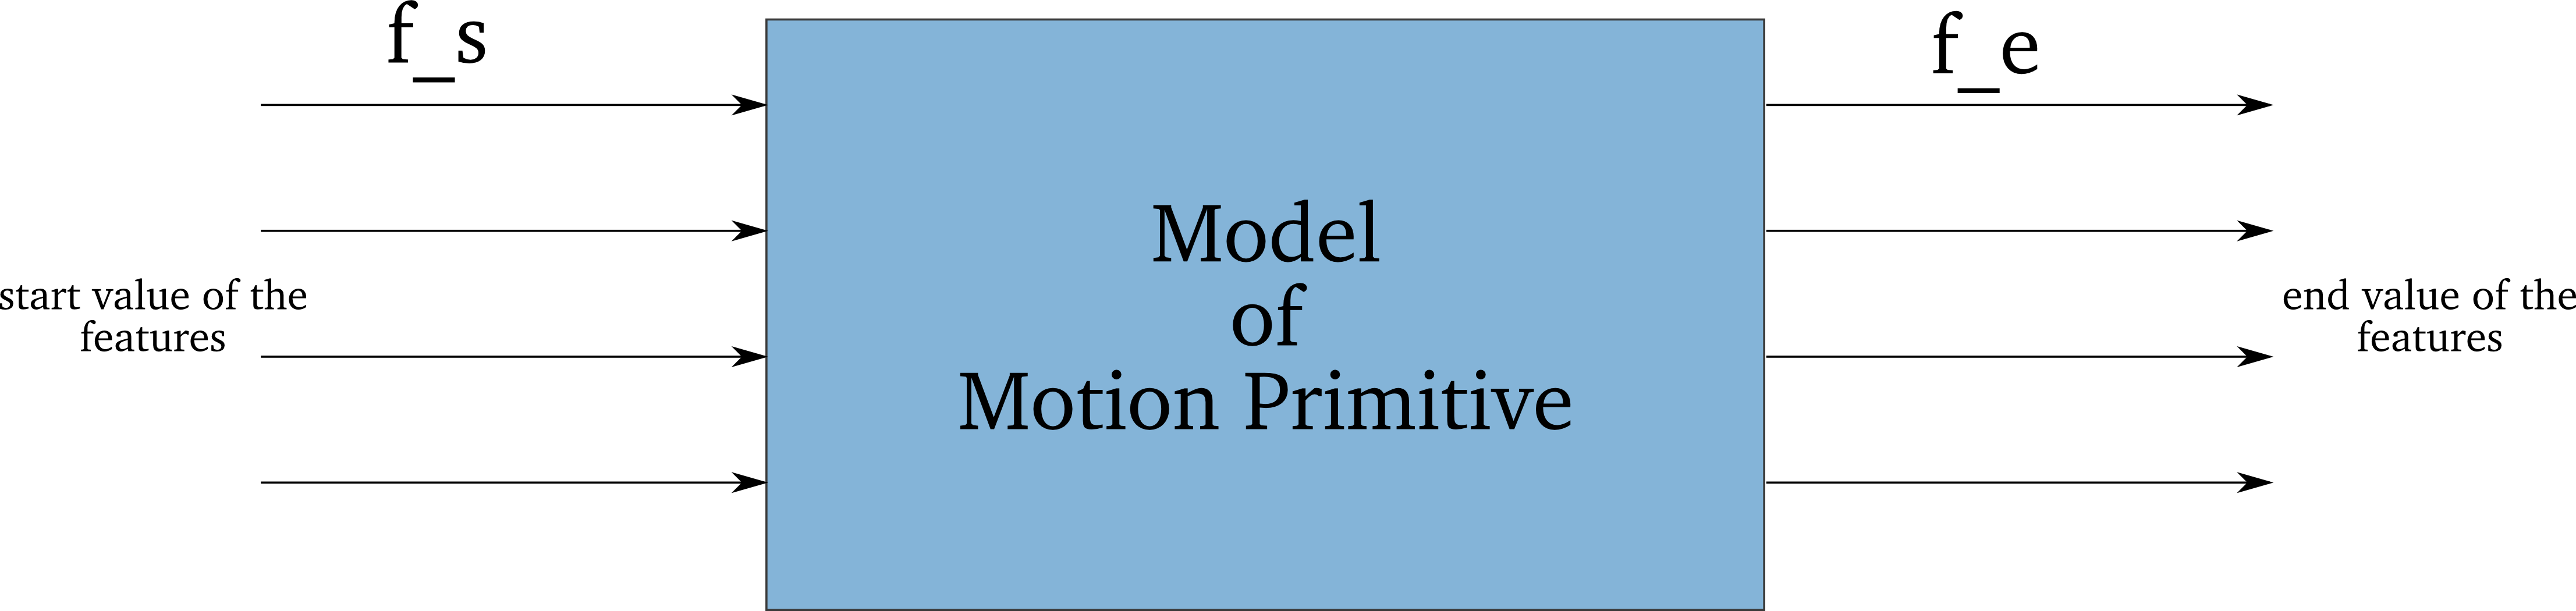
\includegraphics[scale=0.40]{images/model.png}
\caption{Model of motion primitive}
\label{model}
\end{figure}

When the number of training set is limited,learning on
 all the features of the world is not a feasible solutions.
 The approach taken here is to find the relevant features on which the 
learning can be made most effectively.
The prespective adopted in finding the relevant features is that in multiple
demonstrations of the same action, some features will share similar values 
in all the demonstrations. Since we are demonstrating a single action
there has to be consistency in some features of the action.
We need to identify these consistent features and these become the relevant
features. The consistency increases the relevance of the feature to
sucessfully predict from new unseen start states.

We will consider a bivariate probability density function $\phi_i$  by
considering 2 variables, the value of a feature in start of demonstration and
its value at the end of the demonstration.

Let $s_i$ be the $i^{th}$ feature of $f_s$, 
and $e_i$ be the $i^{th}$ feature of $f_e$, \\
The bivariate distribution is given by :
\begin{equation}
    \phi_i(s_i , r_i) = \eta_i I_i ( \lfloor s_i \rfloor, \lfloor e_i \rfloor)
\end{equation}
where operator $\lfloor .  \rfloor$ is  a quantization operator, that returns the bin unit in 
the histogram $I_i$, that corresponds to the feature.

The bi-variate distribution is an appropriate criteria to comment on the
relevance of the feature. Using the distribution we can conclude on the
convergence of the feature. A feature which has converged, the final values
will lie on a straight line in the distribution. If all the final values lie on
a straight line it ensures that whatever maybe the initial value the end values
always remain constant. The constant value in all the demonstration concludes
that the corresponding feature is relevant with respect to the intent of the
motion primitive.
This is explained in the figure \ref{fig:feature distribution}. Higher the
degree of convergence, higher the relevance of the feature for the motion
primitive.
\begin{figure}
    \centering
    \begin{subfigure}[b]{0.4\textwidth}
        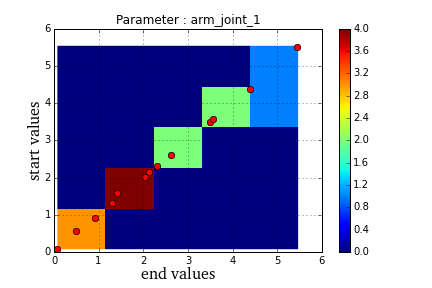
\includegraphics[scale=0.5]{images/arm_joint_1JoinPDF.png} 
        \caption{Distribution of the feature describing arm joint 1.}
        \label{sub fig 1}
    \end{subfigure}
    \begin{subfigure}[b]{0.4\textwidth}
        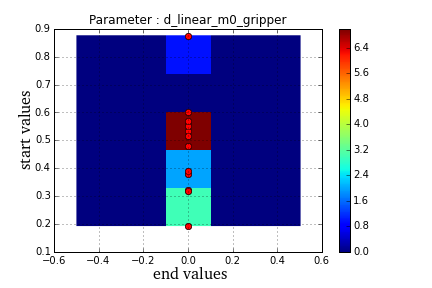
\includegraphics[scale=0.5]{images/d_linear_m0_gripperJoinPDF.png} 
        \caption{Distribution of feature describing distance of object 0 and tooltip. }
        \label{sub fig 2}
    \end{subfigure}
    \caption[Bivariate distribution of features]{An example of bivariate
        distributions of two features for the \textit{move} arm relative to object motion
        primitive.The x-axis is the end values of demonstration while the 
        y-axis is the start value of the demonstration. The dots are the 
        feature values across 12 demonstrations.
        Based on the distribution in \ref{sub fig 1}, we can say that
        there is no certaininty in the end values. This 
        results in lower relvance to the motion primitive . Based on the
        distribution in \ref{sub fig 2},we can say that the end states are
        more concentrated.This ensures that for any value in the start state
        we are sure that the end values always remain same.
        This results in a higher relevance with respect to the motion
    primitive.}\label{fig:feature distribution}
\end{figure}

To calculate this relevance in the distribution, we use two different 
measuring  methods. 1) Entropy 2) Conditional entropy.
We compute the 
entropy $H_i$ and conditional entropy $CH_i$ of the bi-variate distribution $\phi_i(s_i, r_i)$.

Entropy of a discrete random variable is given by,
\begin{equation}
    H(X) = - \sum P(X) \log P(X)
\end{equation}


For a pair of discrete random variables X and Y, which are co related 
conditional entropy of X given Y $h(X|Y)$ is given by :
\begin{equation}
    H(X|Y) =  - \sum _{k = -K}^{K} p_X(x|y) p_Y(y|x) \log \frac{p_Y(y|x)}{p_X(x|y) p_Y(y|x)}
\end{equation}


Based on the entropy or conditional entropy we define the model relevance of a motion primitive.
\begin{equation}
    p(f | \theta ) = \prod_i e^{-E_i}
\end{equation}
where $\theta$ is the set of all $\phi$, and $E_i$ can be $H_i$ or $CH_i$



\subsection{Expert knowledge base}
In our work we create the knowledge base based on expert knowledge of the tasks being performed.
An individual subset of feature space $F$ is called as a template $t$. $t_i \subset F $ .
For example the template $t_1$ contains all the features describing the joint angles of the robot, template $t_2$ contains features which describes 
distance of tooltip to manipulated object.

A collection of the templates is called as a knowledge base $K$.


$K = t_1 \and t_2 \ldots t_n $


\begin{figure}[htp]
\centering
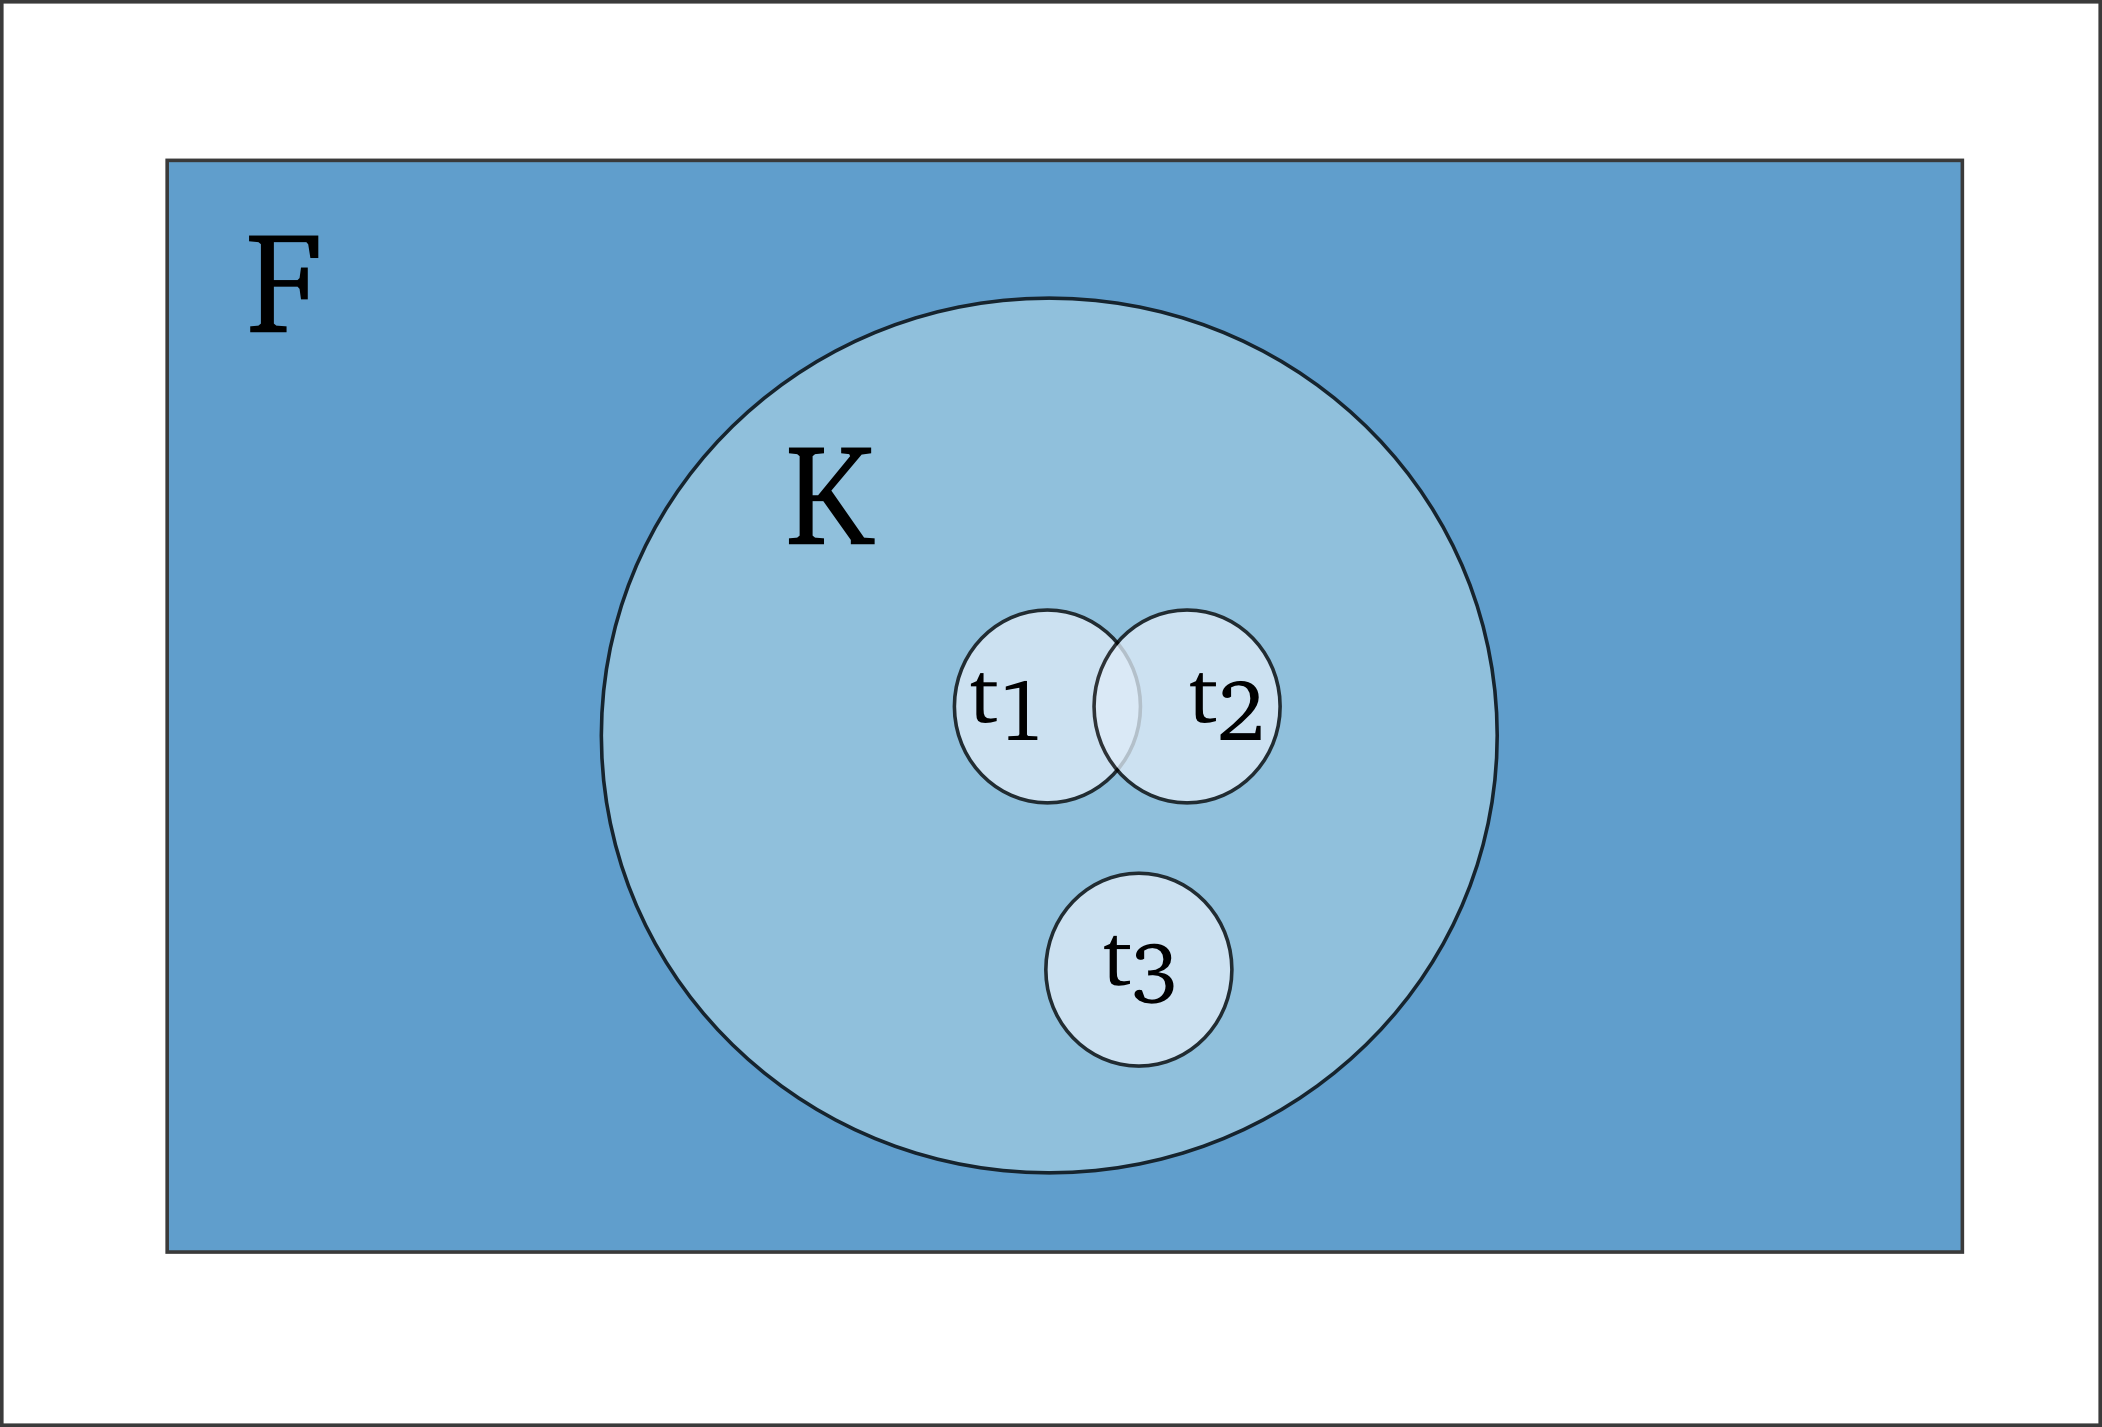
\includegraphics[scale=0.50]{images/feature_space.png}
\caption[Feature space venn diagram]{Relation between feature space F, knowledge base K and the templates t}
\label{}
\end{figure}
Thus for each template $t_i$ we have created a low dimension subset of the feature space $F$.
Our aim is not to find minimum set of features but to find relevant set of features which can describe an action.


The novelty in our approach is the representation of the expert knowledge base.
The knowledge base has been structured using the effect metrics. 
The templates in the knowledge base are organised on the basis of the effect metrics.
The structured nature of the knowledge base helps in determining the relevant features with
less number of demonstrations.
\subsubsection{Effect Metrics}
Effects are defined as changes to the robot-world relationship and/or to positions, orientations
and states of external objects and robot \cite{alissandrakis_action_2006}

In this work we only consider changes to the robot-world relationship and changes to positions, orientations and states of the robot. Based on the orientation and position of the 
robot in environment 2 types of effect metrics can be used, \textit{position} and \textit{orientation}

\begin{figure}[htp]
\centering
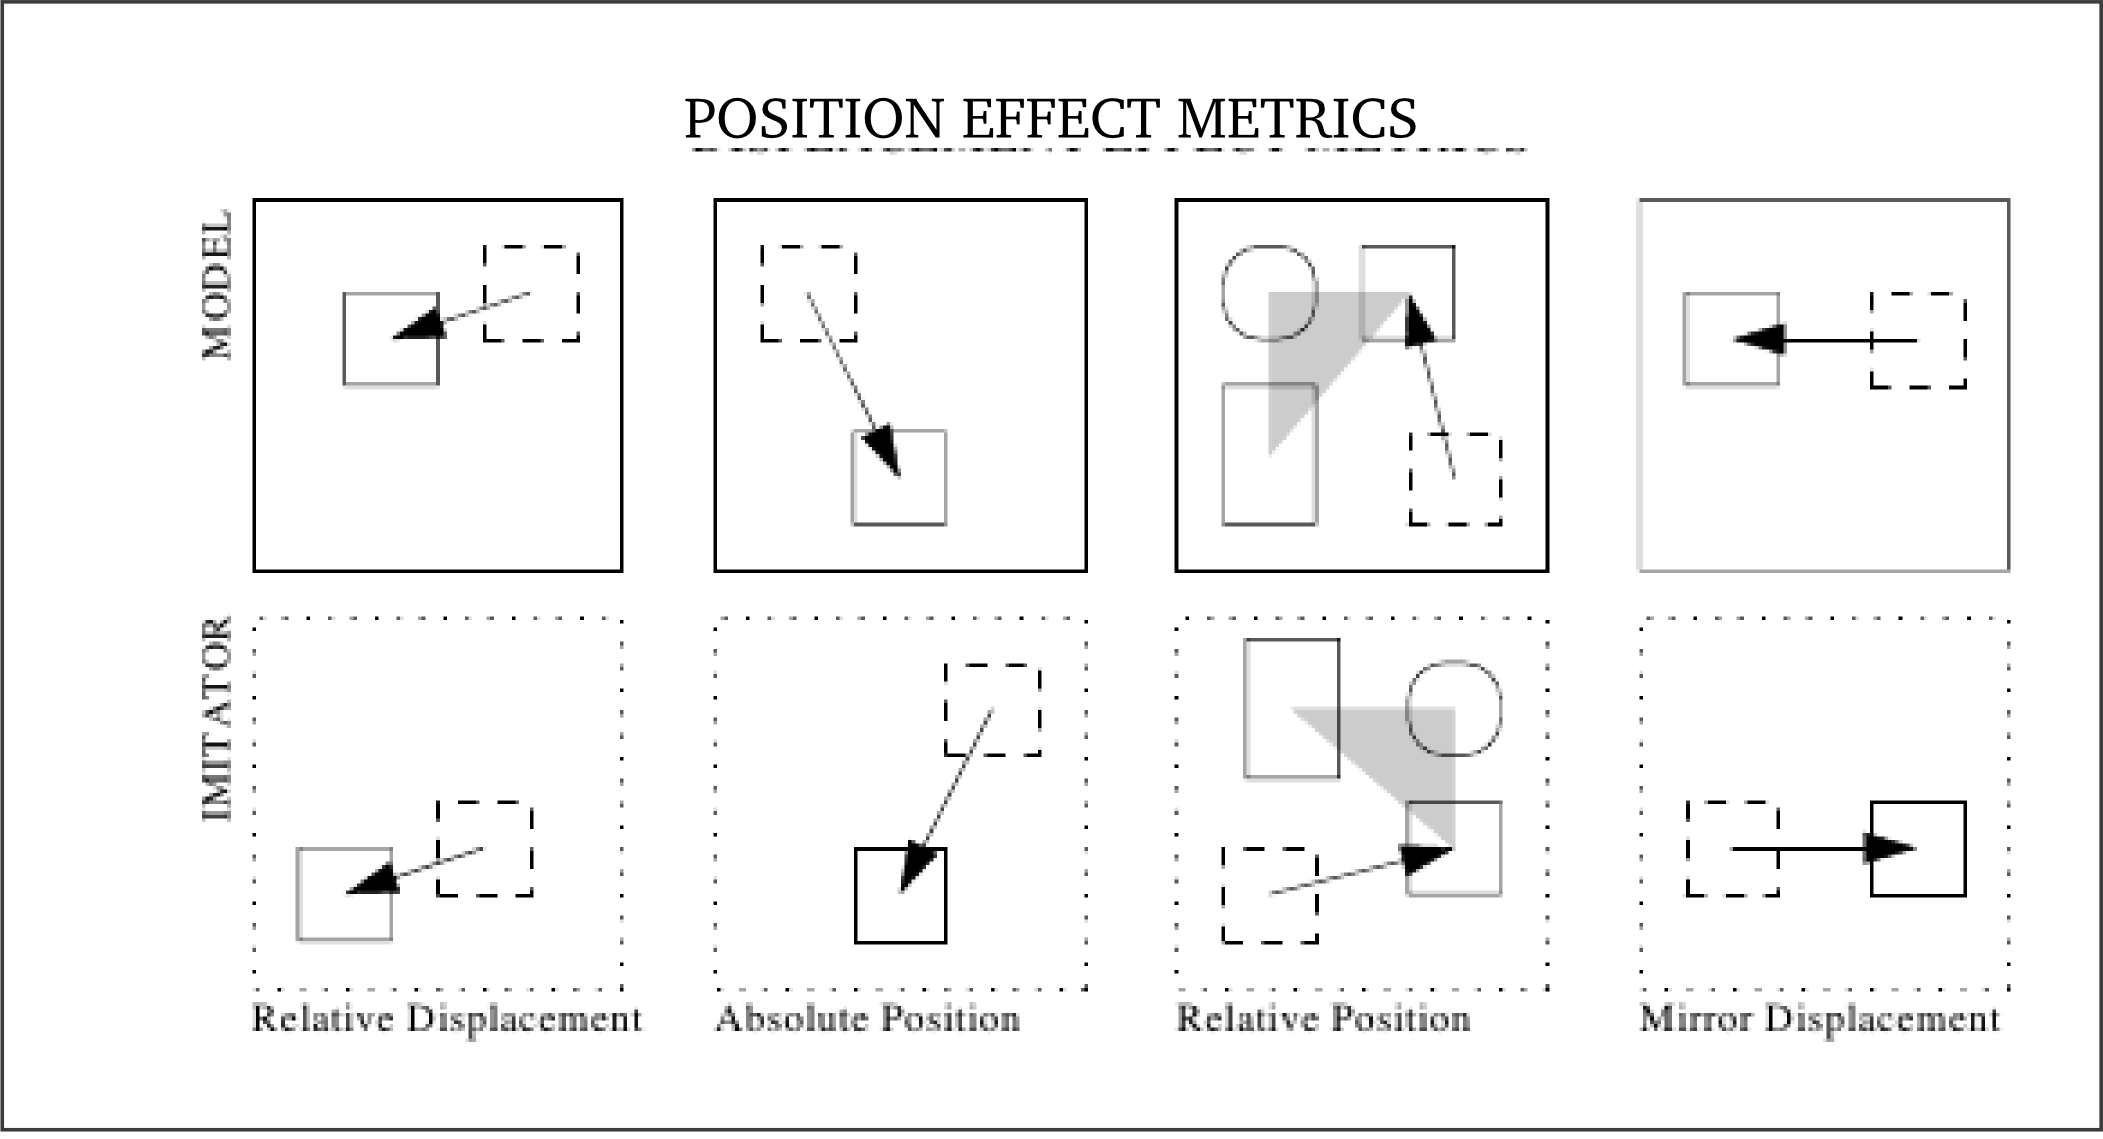
\includegraphics[scale=0.70]{images/position_effect_metrics.png}
\caption[Position effect metrics]{Position effect metrics.
 To measure the change in the relation of change in positions between 
robot and environment objects 
\textit{relative displacement, absolute position, relative position and mirror position}
 effect metrics can be used. First row shows the demonstration and
 their resulting effects. The second rows represents the
 corresponding object (in different workspace ) how it needs to be
 moved (from dashed to solid outline) by an imitator to match the 
corresponding effects according to the metric. The grey triangle
 are superimposed to show the relative position of the objects are 
the same in final state. \cite{alissandrakis_action_2006} }
\label{position effect metrics}
\end{figure}
\begin{figure}[htp]
\centering
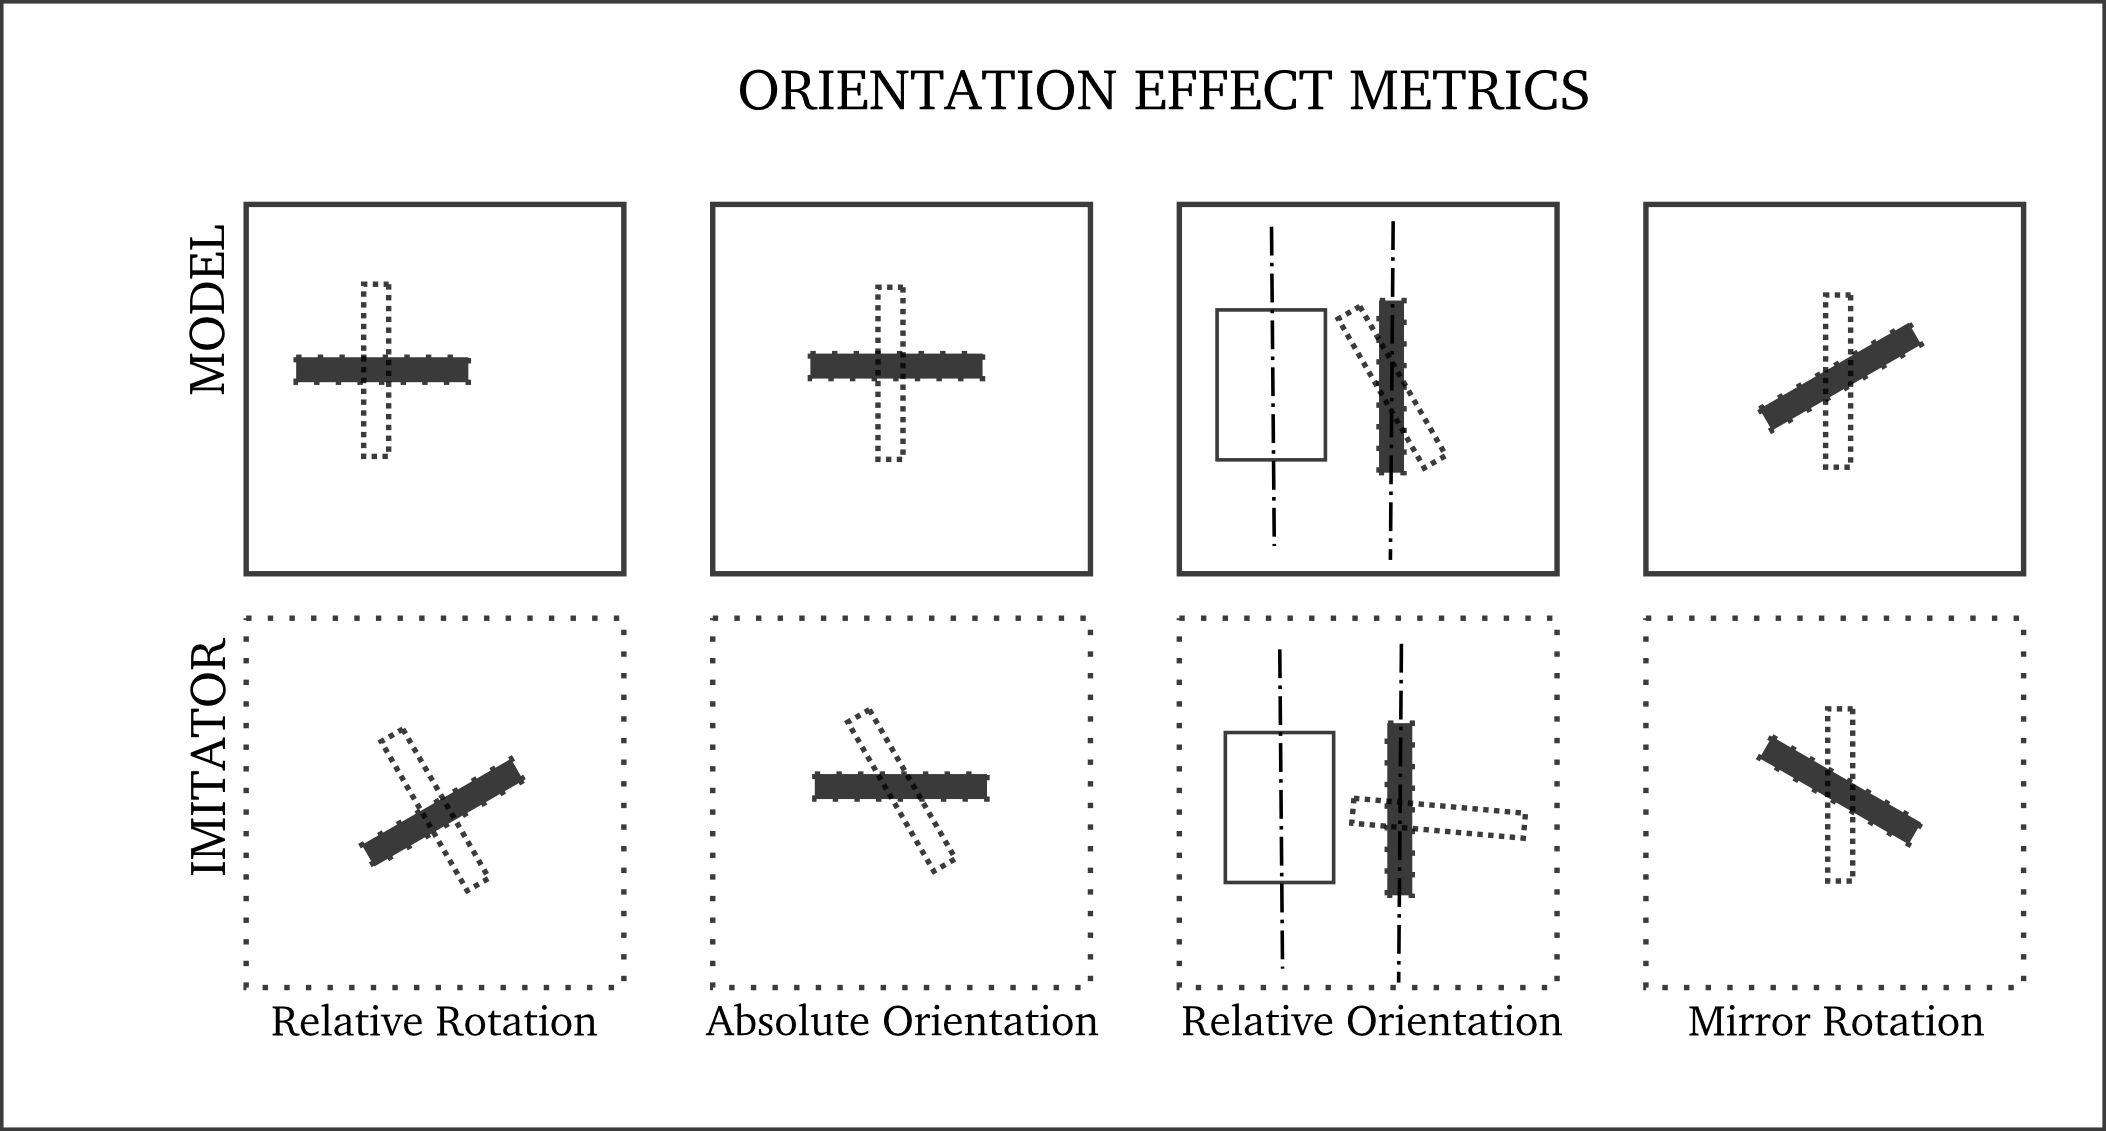
\includegraphics[scale=0.70]{images/angular_effect_metrics.png}
\caption[Orientation effect metrics]{Orientation effect metrics.  To measure the change in the relation of change in orientation between robot and environment objects \textit{relative rotation, absolute orientation, relative orientation and mirror rotation} effect metrics can be used.First row shows the demonstration and their resulting effects. The second rows represents the corresponding object (in different workspace) how it needs to be moved. (from dashed to solid outline) by an imitator to match the corresponding effects according to the metric. The guide lines are superimposed to show the relative orientation of the objects are the same in final state. \cite{ alissandrakis_action_2006}}
\label{orientation effect metrics}
\end{figure}

The different position metrics are 
\begin{itemize}
	\item relative displacement
	\item absolute position
	\item relative position
	\item mirror position
\end{itemize}

the different orientation metrics are 
\begin{itemize}
	\item relative rotation
	\item absolute orientation
	\item relative orientation
	\item mirror rotation
\end{itemize}

Depending on the effect metric the same demonstration can be interpreted as different. 
The example in figure \ref{effect metrics} explains this.
\begin{figure}[htp]
\centering
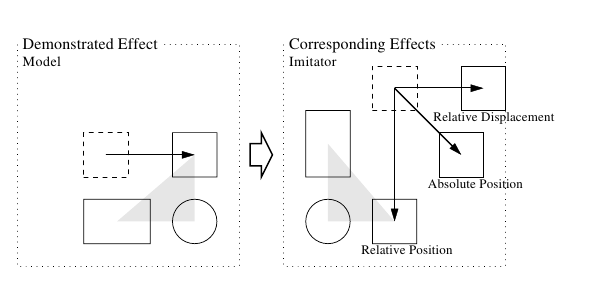
\includegraphics[scale=0.8]{images/effect_position.png}
\caption[Effect metrics in imitation]{The figure illustrates three examples
 of the imitation based on a single demonstration. The left box is the
 demonstrated action. The right box is the possible final state based on
 the position metrics used. The grey triangles are superimposed to show
 the relative distance is maintained \cite{alissandrakis_action_2006}}
\label{effect metrics}
\end{figure}

Based on the effect metrics the knowledge base is organized in different templates which describe an action.
The templates developed in this work are categorized based on the effect metrics.

\subsection{Selecting template from the knowledge base}
For computing the relevance, we use a 3 stage procedure:
\begin{enumerate}
    \item Comparing mean of start value and end value of the feature. $\rightarrow$ To determine that the feature has changed.
            (This was used because features which were not changed in demonstration also have low entropy. So to remove these features this condition 
            check was introduced.)
    \item Comparing the standard deviation of start value and end value of the featue $\rightarrow$ To determing the feature shows convergence in information.
            (This was used because there were features which changed and had low entropy but they were divergent in nature. So to remove the effect of 
            these features this condition check was introduced as explained in figure \ref{fig:box plot})
    \item Calculating the entropy/conditional entropy of the final value of features whose values have changed.
\end{enumerate}

\begin{algorithm}[H]
 \KwData{\\ $f_s$ : start value of the features \\
         $f_e$ : end value of the features\\
        K : knowledge base }
 \KwResult{\\ relevance $L$ of each Template }
 R=0\;
 \For{each template $t$ in K}{
    \For{each feature $f$ in $t$ }{
  read start values $s$ of feature $f$ from $f_s$\;
  read end values $e$ of featue $f$ from $f_e$\;
  \If{mean(s) equals mean(e)}{
       $ R += 1$\;
   }
   \If{standard deviation(s) is less or equal to standard deviation(e)}{
       $ R += 1$\;
   }
    $R += \text{entropy(e)} or\text{ conditional entropy}(e|s)$\;
  }
 }
 \caption{Algorithm for computing relevance of the templates in knowledge base}
\end{algorithm}

\begin{figure}
    \centering
    \begin{subfigure}[b]{0.3\textwidth}
        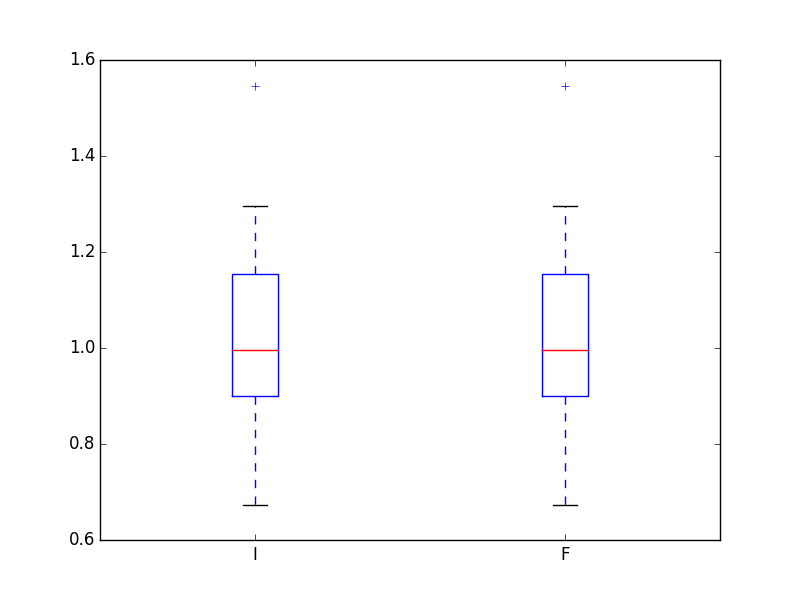
\includegraphics[scale=0.25]{images/boxplot_same_mean.png} 
        \caption{}
        \label{sub box 1}
    \end{subfigure}
    \begin{subfigure}[b]{0.3\textwidth}
        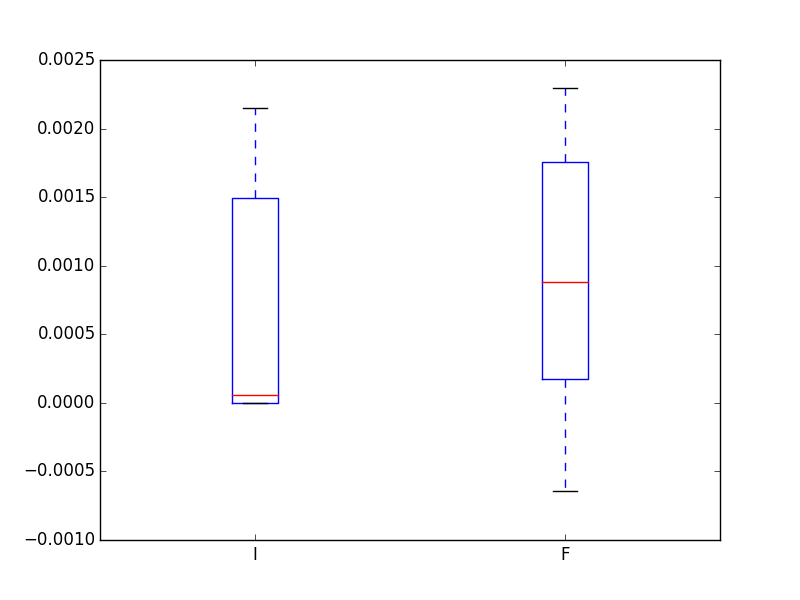
\includegraphics[scale=0.25]{images/boxplot_noconvergence.png} 
        \caption{}
        \label{sub box 2}
    \end{subfigure}
    \begin{subfigure}[b]{0.3\textwidth}
        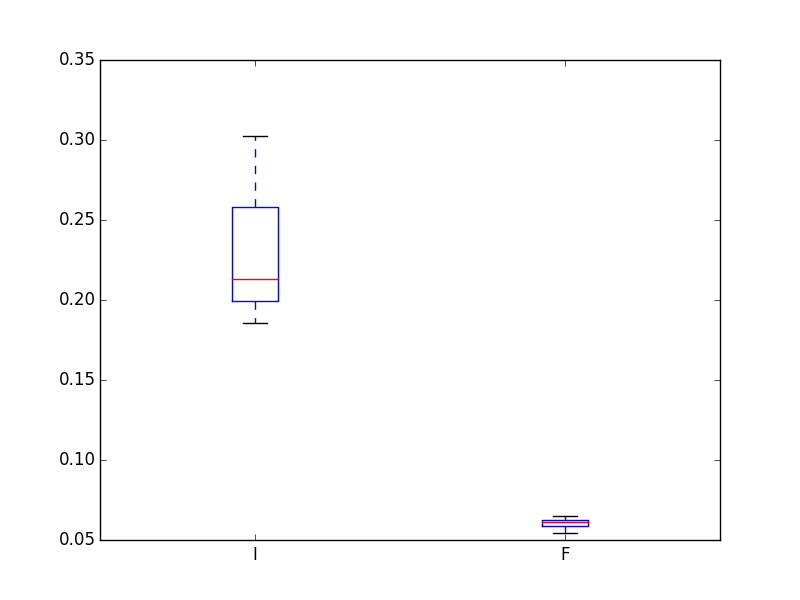
\includegraphics[scale=0.25]{images/boxplot_converged.png} 
        \caption{}
        \label{sub box 3}
    \end{subfigure}
    \caption[Box plot of features]{Box plots of features. Each figure has 2 box plots.
Plot I is of the start value of the feature while plot F is of the end value
of the feature. Figure \ref{sub box 1} is box plot of a featue whose mean values 
have not changed for both start and end values of the feature .
Figure \ref{sub box 2} is the box plot of a feature whose mean value 
has changed but the final values has not converged. 
Figure \ref{sub box 3} is the box plot of a feature whose mean value 
has changed and the final values have converged.} \label{fig:box plot}
\end{figure}


For each $t_i \in K $, we compute a score $\beta_i$ that combines model fitting and the number of 
features in the template.
\begin{equation}
    \beta_i = -2 \log (p (f | \theta_i)) - \alpha_i L_i
\end{equation}
where $\theta_i$ are the distributions related to the features of $t_i$
and $L_i$ is the number of features in the template.
The first term of equation  computes relevance and the second term, weighted by $\alpha$, encourages the usage of templates
consisting of a large number of features $L_i$ .


The most relevant template $T^*$ is selected as :
\begin{equation}
    T^* = \operatornamewithlimits{argmin}_i (\beta_i)
\end{equation}

\newpage
\section{Experiments and Evalutaion}
The proposed motion primitive representation and recommending valid features using modified
knowledge base was validated by learning the \textit{move} motion primitive
on both simulation and on the real robot youBot.

\subsection{Experiment Setup}

The experiments were conducted on data obtained from both simulation as well on
the real robot. The learning of the movement of the base was done in the
simulation software. Gazebo \footnote{http://gazebosim.org/} simulator was used
to simulate the workspace of the robot. The model of the workspace used was
taken from the robocup@work competition
\footnote{http://www.robocupatwork.org/resources.html}. An illustration of the
workspace is shown in figure \ref{gazebo}. The demonstrations of moving the base was done by
teleoperation using a joy-pad.

\begin{figure}[htp]
\centering
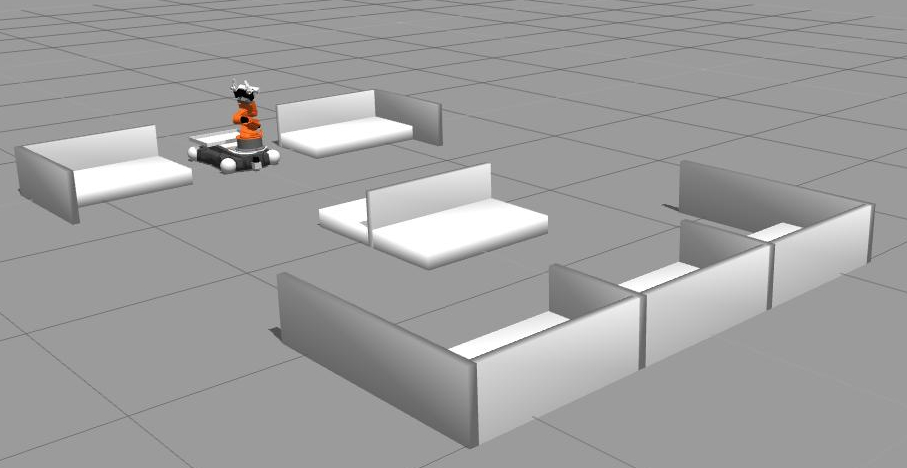
\includegraphics[scale=0.5]{images/gazebo_arena.jpg}
\caption{Gazebo simulator and robocup@work workspace with KUKA youBot}
\label{gazebo}
\end{figure}

The learning of the arm movements was done on the real robot. The robot used
for experimentation is the KUKA youBot \footnotemark.
The youBot has an omnidirectional mobile platform on which a five-axis robot
arm is mounted. The arm was used to teach the move motion primitive .
Kinesthetic demonstrations was used for teaching various arm poses as shown in figure \ref{youBot}.
As we do not address perception in our scope of our work, we used QR markers attached to the objects 
and measured their pose using the camera mounted on the robot's arm.

\begin{figure}[htp]
\centering
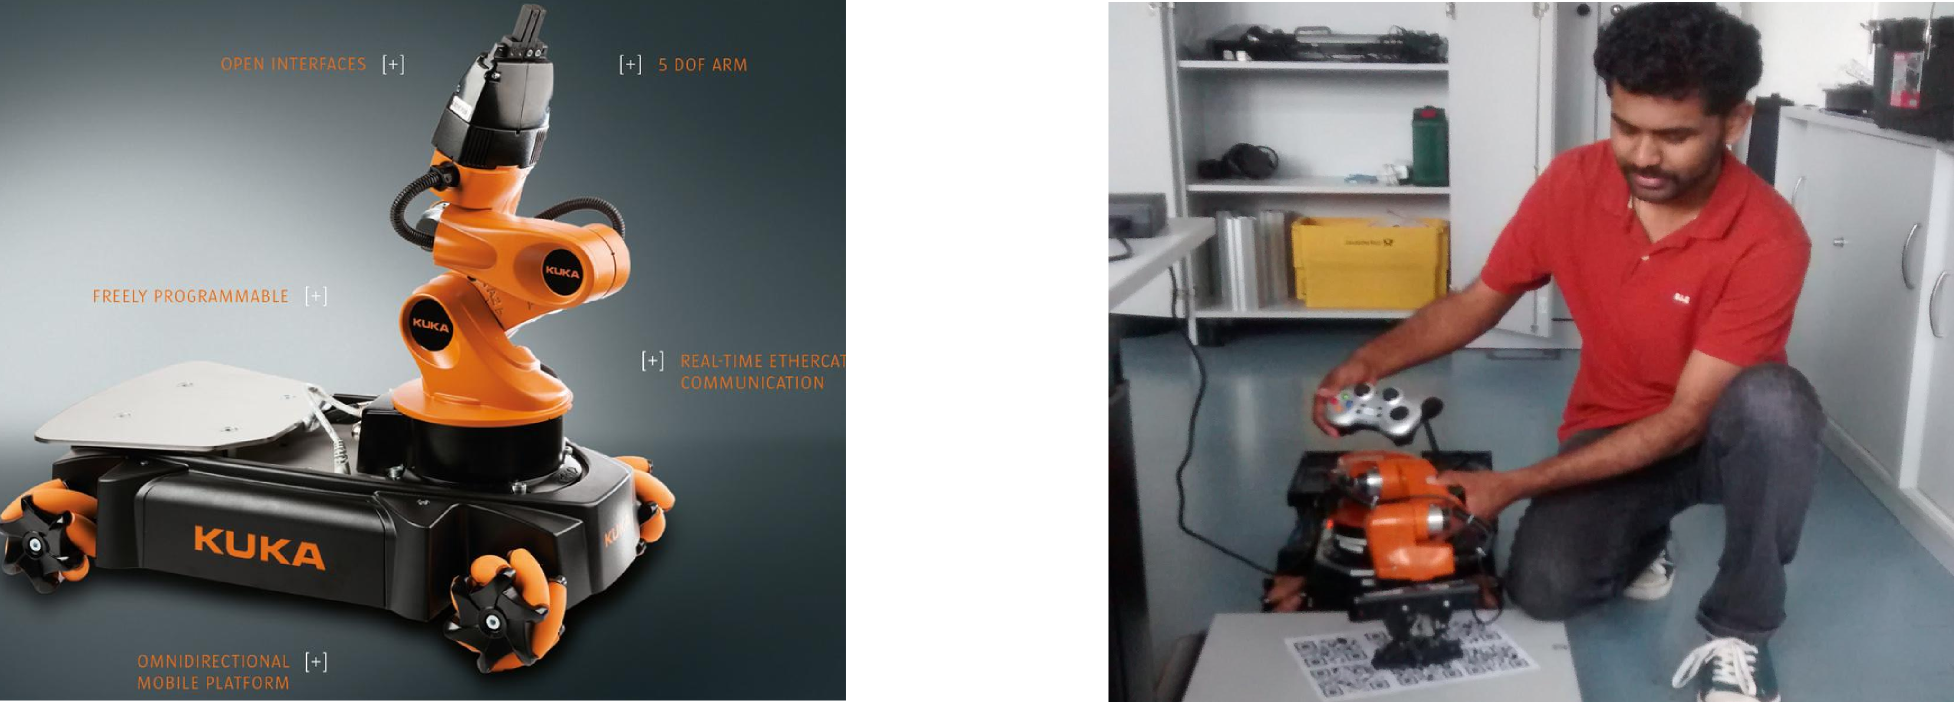
\includegraphics[scale=0.9]{images/kuka_teaching.png}
\caption[KUKA youBot kinesthetic teaching]{a) KUKA youBot \footnotemark . b) The teacher demonstration manipulative motion primitive to the youBot}
\label{youBot}
\end{figure}
\footnotetext{http://www.kuka-robotics.com/germany/en/products/education/youBot/}

\subsubsection{Steps to recording demonstrations}
The demonstrations used for learning consist of two parts.
The first part is the start values and the second part is the end values.
For each demonstration the values of the features are recorded first in the start state and then 
in the end state.
The steps involved in recording the demonstrations is explained in the figure \ref{record demonstration}
\begin{figure}[!htp]
\centering
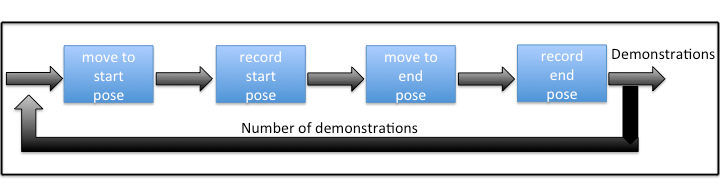
\includegraphics[scale=0.5]{images/record_readings.png}
\caption[Recording demonstrations]{Steps involved in recording the demonstrations}
\label{record demonstration}
\end{figure}


\FloatBarrier
\subsection{Experiments}
The experiments conducted for the work were to teach
some of the motion primitives related to the tasks in RoboCup@Work competition.

\subsubsection{RoboCup@Work}
Robocup@work competition \footnote{http://www.robocupatwork.org/} is conducted on various tasks, which are involved in work-related scenarios.
The tasks involved in the competition are taken directly from a list of scientifically and industrial
challenges. The table \ref{robocup task} list the various test conducted during the competition. In our
experiments we tried to learn the motion primitives related to the task executed in the competition.
\begin{table}[htdp]
    \begin{center}
\begin{tabular}{|l|p{8cm}|}
    \hline
    \textbf{Task} & \textbf{Description}\\
    \hline
    Basic Navigation Test &  can the robots navigate well in their environment, i.e. in a goal-oriented, autonomous, robust, and safe way\\
    \hline
    Basic Manipulation Test& demonstrate basic manipulation capabilities by the robots, like grasping, turning, or placing an object\\
    \hline
    Basic Transportation Test &  assess the ability of the robots for combined navigation and manipulation tasks\\
    \hline
    Precision Placement Test  &  drop objects precisely into cavities\\
    \hline
\end{tabular}
\end{center}

\caption{Robocup Task list}
\label{robocup task}
\end{table}

\subsubsection{Motion primitives learnt }
The motion primitives which were learnt for validating the approach are as follows
\begin{enumerate}
    \item \textit{move} base to absolute pose
    \item \textit{move} base to relative pose to object
    \item \textit{move} arm to absolute pose
    \item \textit{move} arm to relative pose to object
\end{enumerate}

\FloatBarrier
\subsection{\textit{move} Motion Primitive}
The \textit{move} motion primitive is an important building block for all the
skills used in an industrial setup.  For example lets consider the
'pick up' skill in an industrial setup. This skill can be fragmented into the following motion
primitives:
\begin{itemize}
    \item \textbf{pick up skill :}
\begin{enumerate}
    \setlength\itemsep{0.1em}
    \item \textit{move} base to platform
    \item \textit{move} arm to "look platform" pose
    \item locate objects
    \item \textit{move} arm to pre-grasp pose
    \item grasp
    \item \textit{move} arm to post-grasp pose
\end{enumerate}
\end{itemize}
\begin{figure}[htp]
\centering
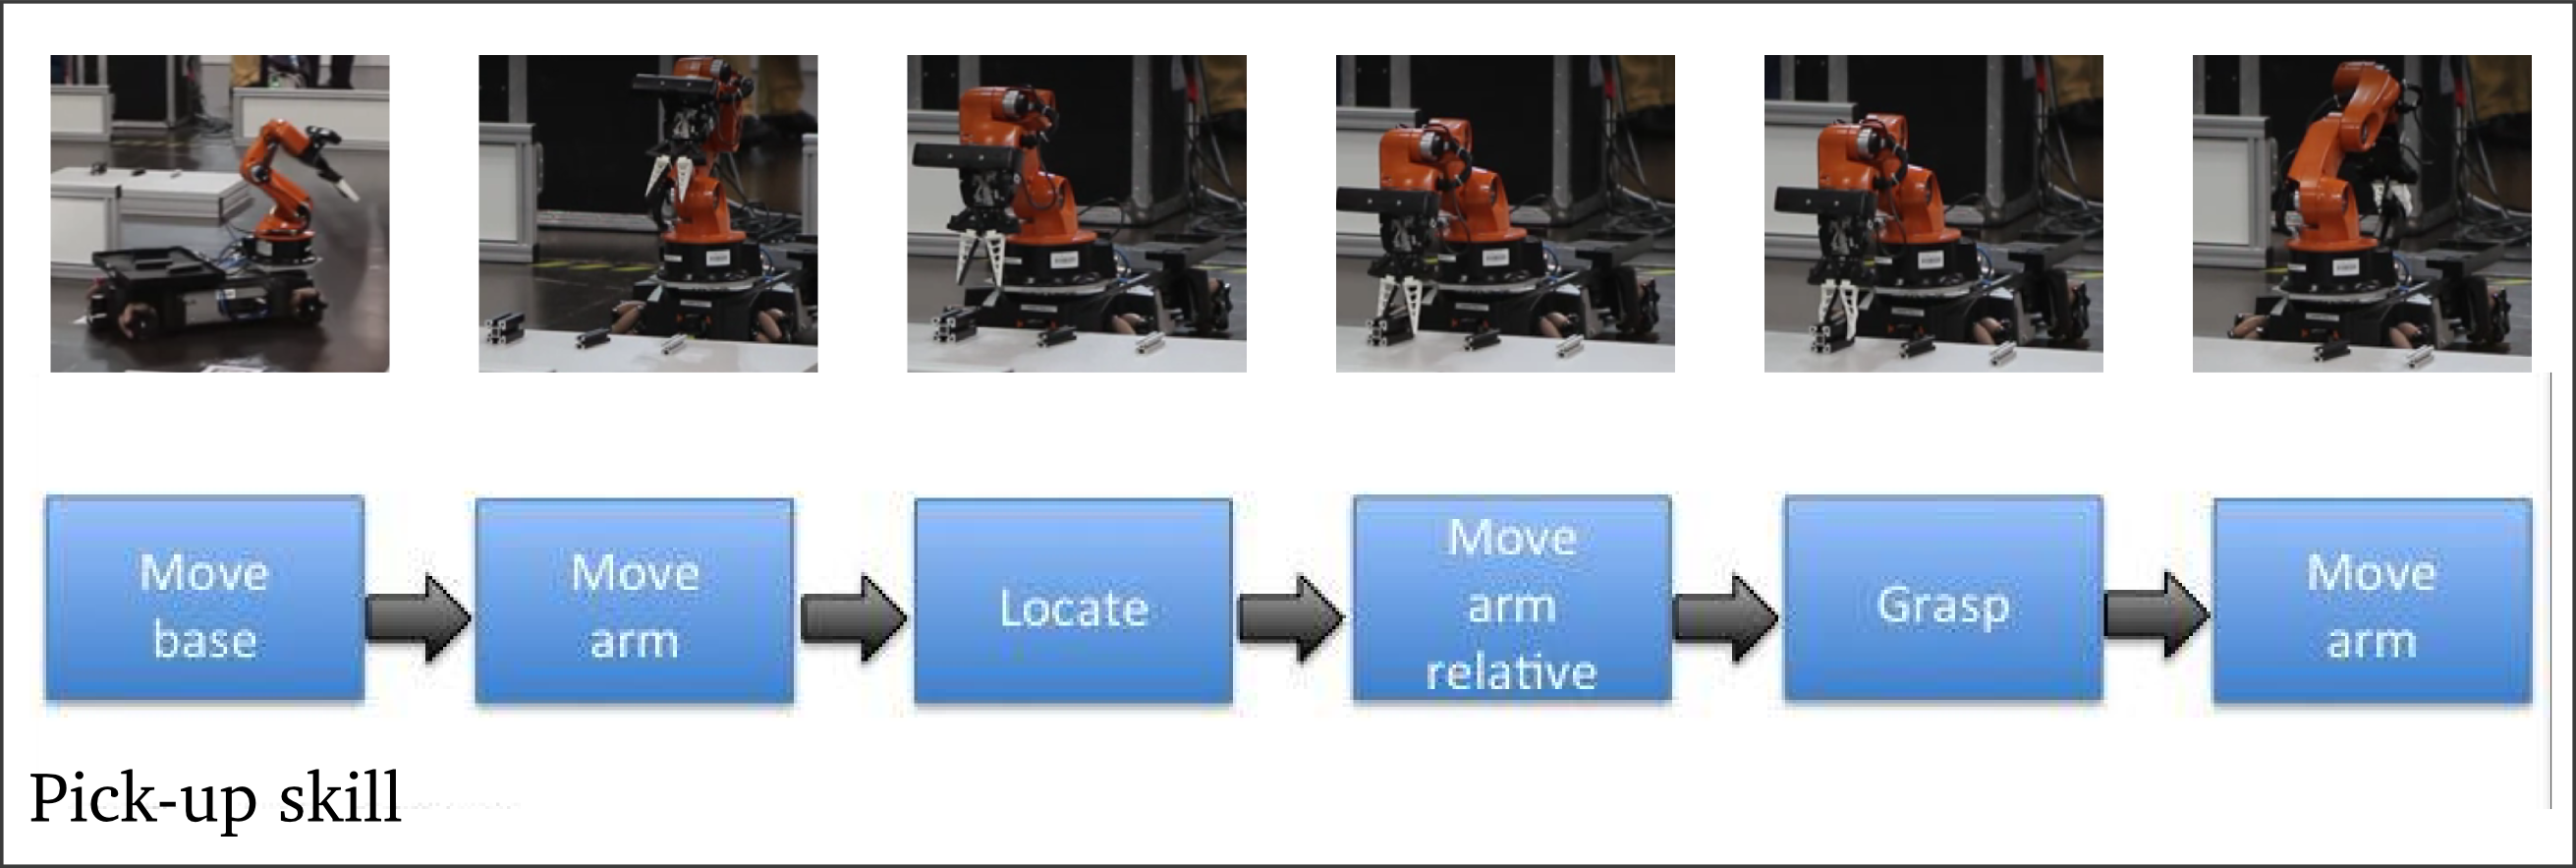
\includegraphics[scale=0.8]{images/pickupskill/pickupskill.png}
\caption['Pick up' skill]{'Pick up' skill : The pick up skill consist of a series of motion primitives. 
The motion primitives and their sequence for executing 'pick up' skill. Images courtesy b-it bots robocup@work (German open 2015)}
\label{pick up}
\end{figure}

The \textit{move} motion primitive can be broadly classified for a mobile manipulator for 2 purposes.
\begin{enumerate}
    \setlength\itemsep{0.1em}
    \item Base movements
    \item Arm movements
\end{enumerate}

The \textit{move} motion primitive can be further classified based on the effect metrics
\begin{enumerate}
    \setlength\itemsep{0.1em}
    \item Absolute pose
        \begin{itemize}
            \item position
            \item orientation
        \end{itemize}
    \item Relative pose
        \begin{itemize}
            \item position
            \item orientation
        \end{itemize}
    \item Relative displacement
\end{enumerate}




\subsubsection{\textit{move} Knowledge base}
The template as defined earlier is a subset of the feature space, which defines
a particular motion primitive. A collection of templates, form the knowledge
base for a particular robot. The templates formulated for the \textit{move} 
motion primitive in youBot are mentioned in the table \ref{knowledge base}

\newcommand{\TemplateA} {joint 1, joint 2, joint 3, joint 4, joint 5}
\newcommand{\TemplateADescription} {Joint angles of the youBot}
\newcommand{\TemplateB} {tooltip link }
\newcommand{\TemplateBDescription} { tool tip frame of youBot}
\newcommand{\TemplateC} { tooltip link, object 1}
\newcommand{\TemplateCaDescription} { Relative distance between pose of tooltip and object 1}
\newcommand{\TemplateCbDescription} { Relative distance between position of tooltip and object 1}
\newcommand{\TemplateCcDescription} { Relative distance between orientation of tooltip and object 1}
\newcommand{\TemplateD} { tooltip link, object 2}
\newcommand{\TemplateDaDescription} { Relative distance between pose of tooltip and object 2}
\newcommand{\TemplateDbDescription} { Relative distance between position of tooltip and object 2}
\newcommand{\TemplateDcDescription} { Relative distance between orientation of tooltip and object 2}

\newcommand{\TemplateE} { tooltip link, object 1, object 2}
\newcommand{\TemplateEaDescription} { Relative distance between pose of tooltip and object 1, object 2}
\newcommand{\TemplateEbDescription} { Relative distance between position of tooltip and object 1, object 2}
\newcommand{\TemplateEcDescription} { Relative distance between orientation of tooltip and object 1, object 2}

\newcommand{\TemplateF} {base link }
\newcommand{\TemplateFDescription} { base link frame of youBot}
\newcommand{\TemplateG} { base link, object 1}
\newcommand{\TemplateGaDescription} { Relative distance between pose of base and object 1}
\newcommand{\TemplateGbDescription} { Relative distance between position of base and object 1}
\newcommand{\TemplateGcDescription} { Relative distance between orientation of base and object 1}
\newcommand{\TemplateH} { base link, object 2}
\newcommand{\TemplateHaDescription} { Relative distance between pose of base and object 2}
\newcommand{\TemplateHbDescription} { Relative distance between position of base and object 2}
\newcommand{\TemplateHcDescription} { Relative distance between orientation of base and object 2}

\newcommand{\TemplateI} { base link, object 1, object 2}
\newcommand{\TemplateIaDescription} { Relative distance between pose of base and object 1, object 2}
\newcommand{\TemplateIbDescription} { Relative distance between position of base and object 1, object 2}
\newcommand{\TemplateIcDescription} { Relative distance between orientation of base and object 1, object 2}

\setlength{\tabcolsep}{6pt}
\renewcommand{\arraystretch}{0.8}

\begin{table}[htdp]
\begin{center}
\begin{tabular}{|c|c|c|p{5cm}|p{5cm}|}
\hline
\multicolumn{5}{ |c| }{\textit{move} Knowledge Base} \\
\hline
	part & metric & type & features & description\\
\hline
	 \multirow{13}{*}{arm} & \multirow{4}{*}{absolute} & position & \TemplateA & \TemplateADescription \\
\cline{3-5}
	 &  & position & \TemplateB & \TemplateBDescription\\
\cline{3-5}
	 &  & orientation & \TemplateB & \TemplateBDescription\\
\cline{3-5}
	 &  & pose & \TemplateB & \TemplateBDescription\\
\cline{2-5}
	 & \multirow{9}{*}{relative} & position & \TemplateC & \TemplateCbDescription\\
\cline{3-5}
	 &  & orientation & \TemplateC & \TemplateCcDescription\\
\cline{3-5}
	 &  & pose & \TemplateC & \TemplateCaDescription\\
\cline{3-5}
	 &  & position & \TemplateD & \TemplateDbDescription\\
\cline{3-5}
	 &  & orientation & \TemplateD & \TemplateDcDescription\\
\cline{3-5}
	 &  & pose & \TemplateD & \TemplateDaDescription\\
\cline{3-5}
	 &  & position & \TemplateE & \TemplateEbDescription\\
\cline{3-5}
	 &  & orientation & \TemplateE & \TemplateEcDescription\\
\cline{3-5}
	 &  & pose & \TemplateE & \TemplateEaDescription\\

\cline{3-5}
	 &  & displacement & \TemplateB & \TemplateBDescription\\
\hline


	 \multirow{12}{*}{base} & \multirow{2}{*}{absolute} & position & \TemplateF & \TemplateFDescription \\
\cline{3-5}
	 &  & orientation & \TemplateF & \TemplateFDescription\\
\cline{3-5}
	 &  & pose & \TemplateF & \TemplateFDescription\\
\cline{2-5}
	 & \multirow{9}{*}{relative} & position & \TemplateG & \TemplateGbDescription\\
\cline{3-5}
	 &  & orientation & \TemplateG & \TemplateGcDescription\\
\cline{3-5}
	 &  & pose & \TemplateG & \TemplateGaDescription\\
\cline{3-5}
	 &  & position & \TemplateH & \TemplateHbDescription\\
\cline{3-5}
	 &  & orientation & \TemplateH & \TemplateHcDescription\\
\cline{3-5}
	 &  & pose & \TemplateH & \TemplateHaDescription\\
\cline{3-5}
	 &  & position & \TemplateI & \TemplateIbDescription\\
\cline{3-5}
	 &  & orientation & \TemplateI & \TemplateIcDescription\\
\cline{3-5}
	 &  & pose & \TemplateI & \TemplateIaDescription\\

\cline{3-5}
	 &  & displacement & \TemplateF & \TemplateFDescription\\
\hline
\end{tabular}
\end{center}

\caption{Knowledge base for \textit{move} motion primitive}
\label{knowledge base}
\end{table}

\subsection{Evaluation metrics}
We designed a dataset to quantitatively evaluated the performance of the 
recommendations made by our algorithm. An expert labeled the templates in
the knowledge base on a 3 point Likert scale of 1-3 (where 3 is the best) 
on the basis of the his expert knowledge. We use this metrics to quantify 
the quality of a ranked list of recommendations by its \acrfull{ndcg} 
\cite{manning_introduction_2008} at positions 1 and 3.
\acrshort{ndcg}@1 is suitable metric for \acrshort{lfd} since we
use the top recommendation for finding our goal.
We consider \acrshort{ndcg}@3 suitable for evaluating the quality of the 
recommendations.

\subsection{Results and Discussions}
This section summarizes the evaluation of our approach conducted using 
kinesthetic demonstrations of the \textit{move} motion primitive.

\subsubsection{\textit{move} base absolute pose}
In this experiment the youBot is
taught to \textit{move} base to an absolute location in the workspace.
The experiments consist of recording different poses of the robot in the workspace.
First the robot is moved to any arbitary position and the start pose is recorded then 
the robot is moved to the intended final position which needs to be taught and the end 
pose is recorded. The above steps are repeated till all the observations are recorded as shown in figure \ref{base absolute exp}.
The motion primitive can be used as a part of the "basic navigation test" task. In these
task the robot has to go to pre-defined locations in the workspace.
We ran the experiments using different number of demonstrations and using both entropy 
and conditional entropy for measuring relevance. The success of the experiments are 
shown in figure \ref{base absolute result}. 
The template describing the pose of the base of the youBot was recommended as the most
relevant template from the demonstrations.

\begin{figure}[htp]
\centering
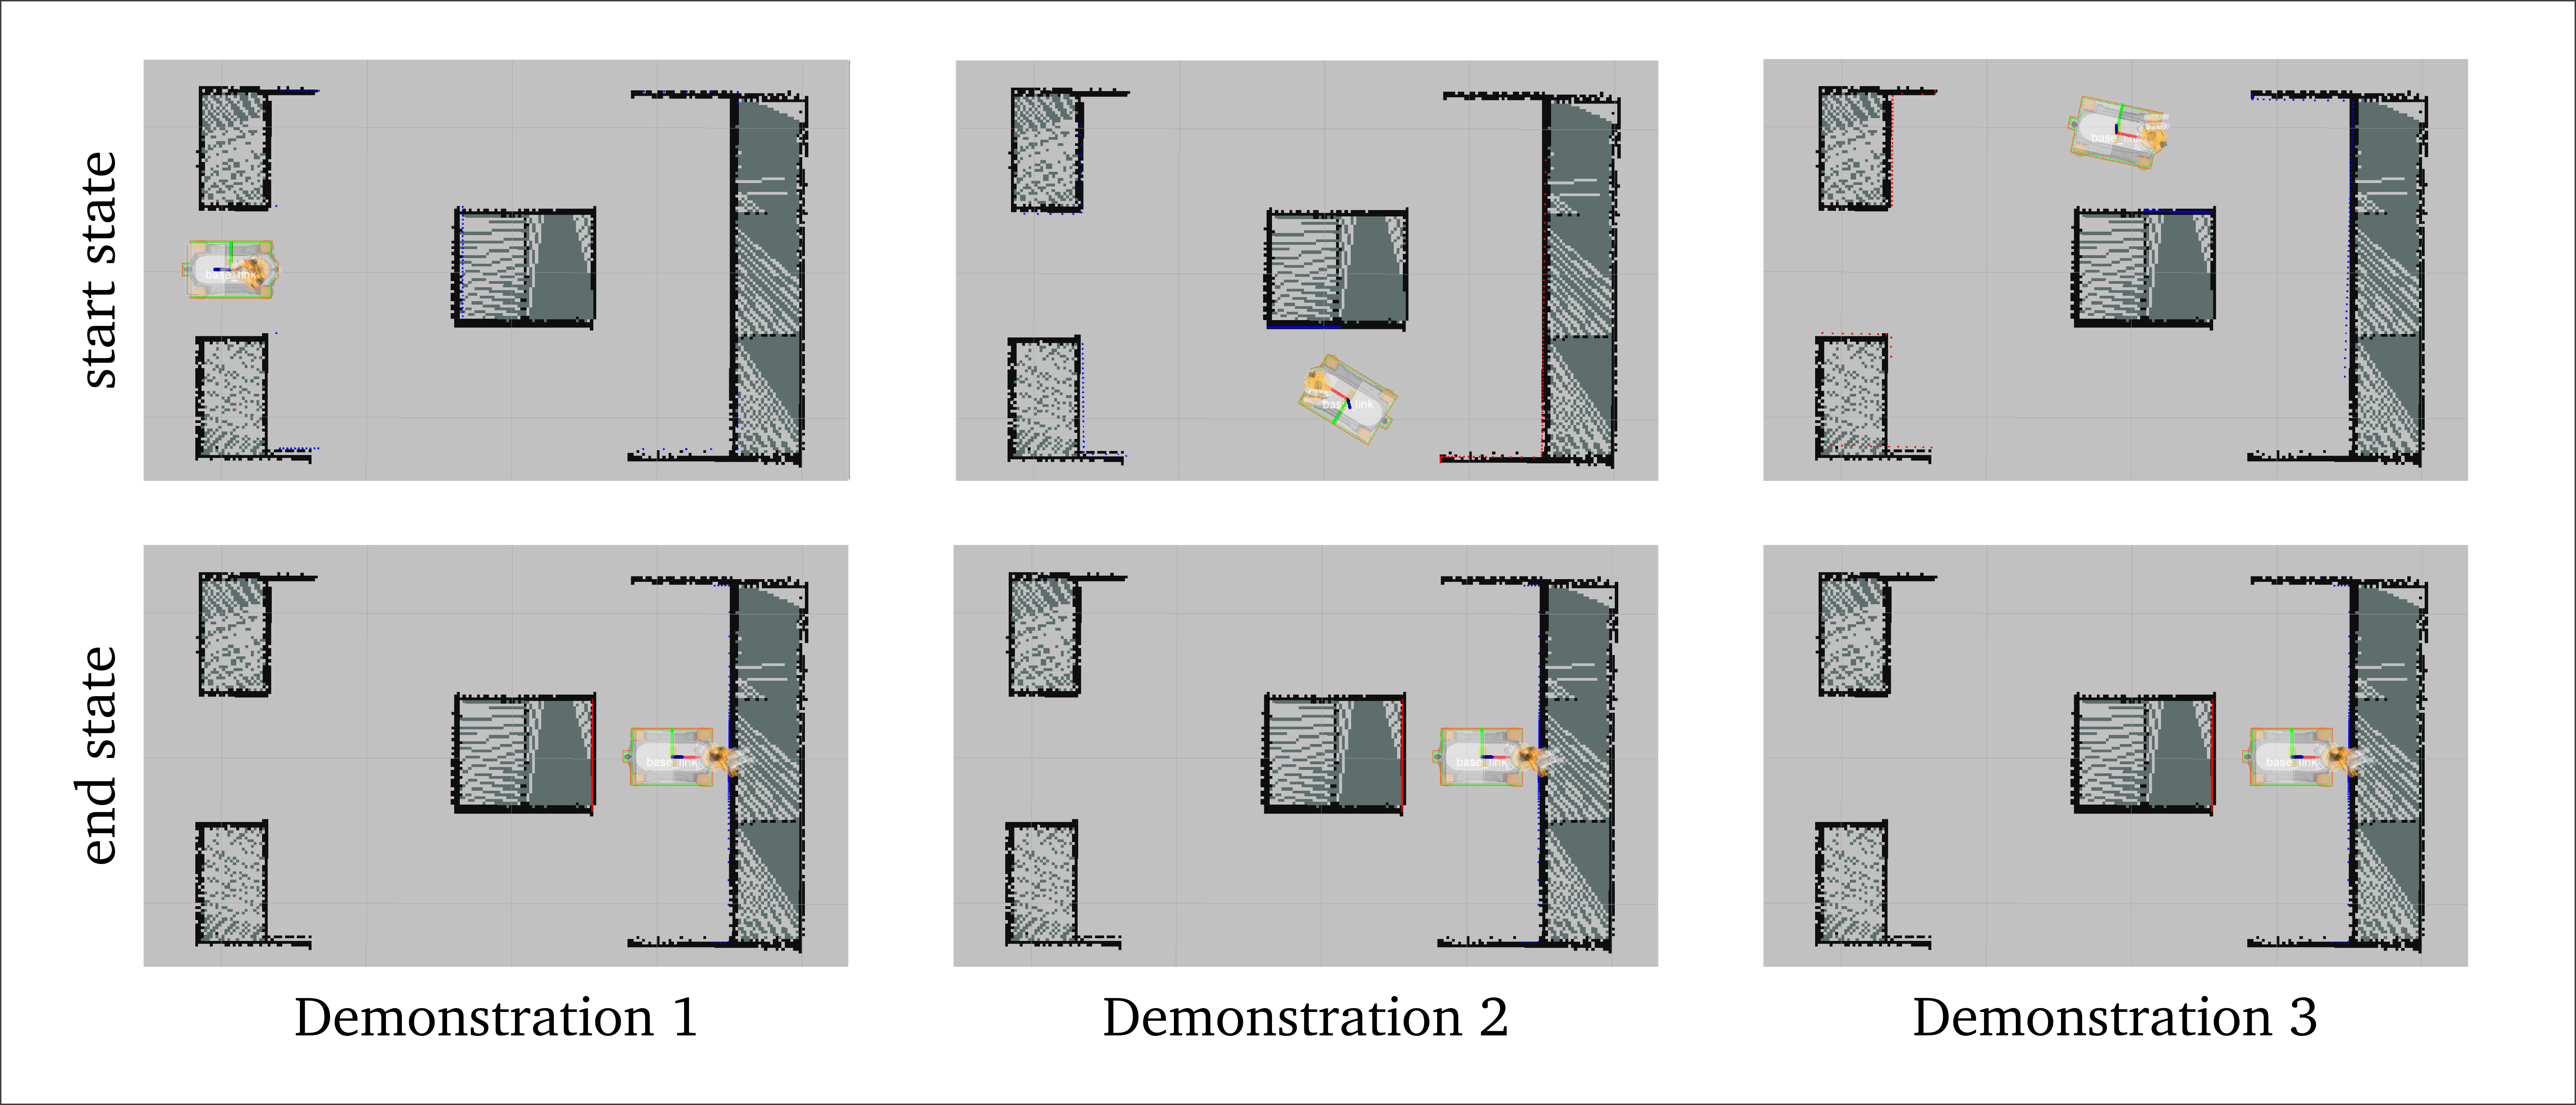
\includegraphics[scale=0.3]{images/base_absolute_exp.png}
\caption[Demonstrations to teach the youBot to move base to an absolute location]
{Demonstrations for teaching the robot to \textit{move} base
to an absolute pose in the workspace. The rows show the recorded start pose and the end pose. The 
columns show the different demonstrations}
\label{base absolute exp}
\end{figure}
\begin{figure}[htp]
\centering
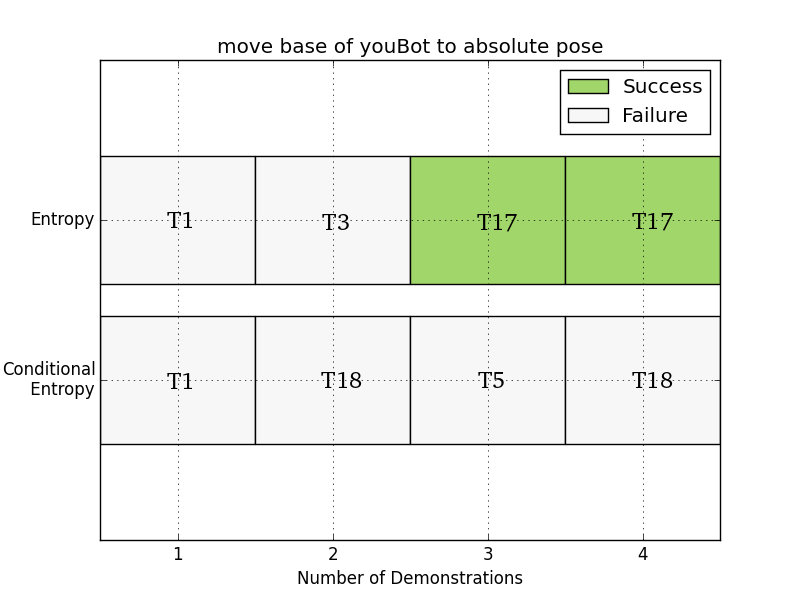
\includegraphics[scale=0.5]{images/base_absolute_result.png}
\caption[Result : \textit{move} base absolute pose]{Results for \textit{ move}
base to an absolute pose. The x-axis denotes the number of demonstrations used
for learning. The y-axis denotes the method used for computing relevance.Each
box is marked with the selected template name. Green
color denotes the relavant template was successfully recommended}
\label{base absolute result}
\end{figure}


\FloatBarrier
\subsubsection{\textit{move} base relative pose to object }
In this experiment the youBot is taught to \textit{move} base to a relative
location in the workspace. The experiments consist of recording different start
and end poses of the robot in the workspace. First the robot is moved to any
arbitary position and the start pose is recorded then the robot is moved to the
intended final position which needs to be taught and the end pose is recorded.
The above steps are repeated till all the observations are recorded as
displayed in figure \href{base relative exp}.
As you can see the object was placed on different platform on each demonstrations.

This particular motion primitive
can be used as a part of the "basic manipulation test" task. In these task the
robot has to go near a platform containing an object. We ran the experiments
using different number of demonstrations and using both entropy and conditional
entropy for measuring relevance. The success of the experiments are shown in
figure \ref{base relative result}. The template describing the relative
distance between the base of youBot and the object was recommended as the most
relevant template from the demonstrations.

\begin{figure}[htp]
\centering
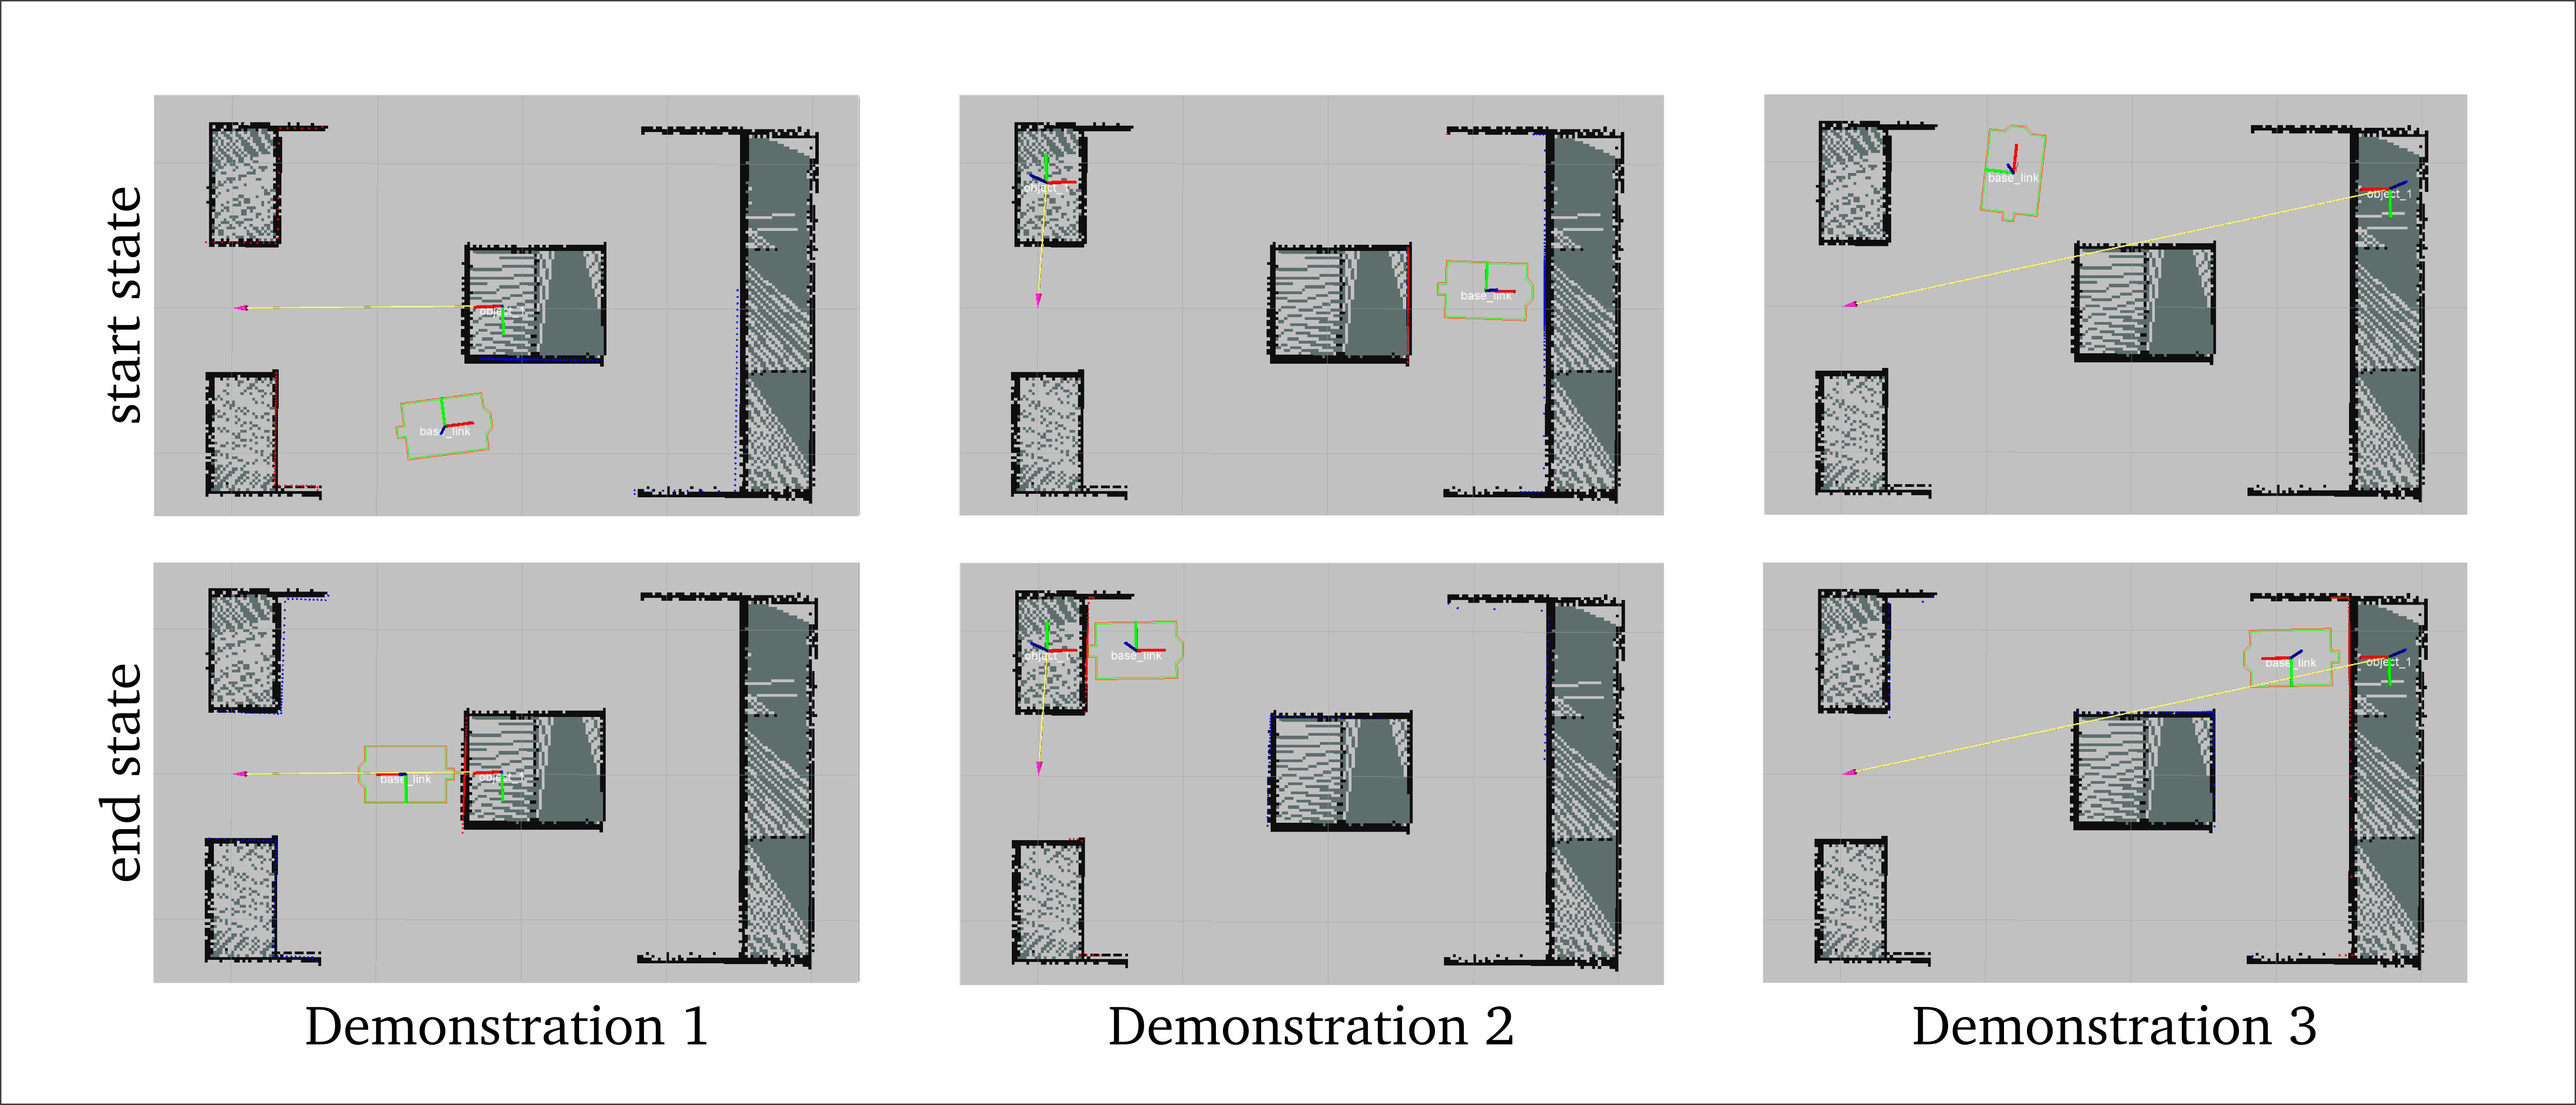
\includegraphics[scale=0.3]{images/base_relative_exp.png}
\caption[Demonstrations to teach the robot to move base to a relative location]
{Demonstrations for teaching the robot to \textit{move} base
to a relative pose in the workspace. The rows show the recorded start pose and the end pose. The 
columns show the different demonstrations}
\label{base relative exp}
\end{figure}
\begin{figure}[htp]
\centering
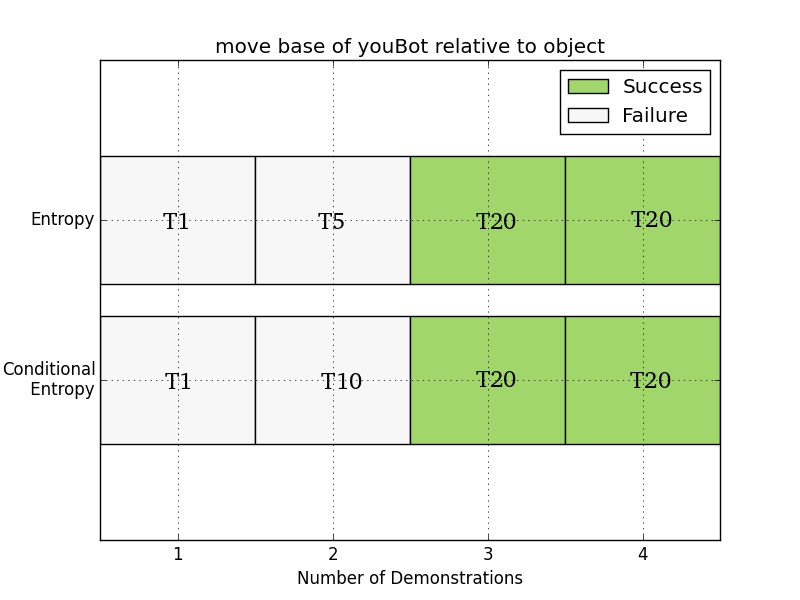
\includegraphics[scale=0.5]{images/base_relative_result.png}
\caption[Result : \textit{move} base relative pose to object  ]{Results for \textit{ move} base to a relative pose. The x-axis denotes the 
number of demonstrations used for learning. The y-axis denotes the method used for 
computing relevance.Each
box is marked with the selected template name. Green color denotes the relavant template was successfully recommended}
\label{base relative result}
\end{figure}

\FloatBarrier
\subsubsection{\textit{move} arm absolute pose}
In this experiment the youBot is
taught to \textit{move} arm to an absolute pose.
The experiments consist of recording different start and end poses of the robot arm. 
First the robot arm is moved to any arbitary position and the start pose is recorded then 
the robot arm is moved to the intended final position which needs to be taught and the end 
pose is recorded. The above steps are repeated till all the observations are recorded as shown in figure \ref{arm absolute exp}


This particular motion primitive can be used as a part of the "basic manipulation test" task. In these
task the robot has to be taught the "look platform" pose for looking at the platform.
We ran the experiments using different number of demonstrations and using both entropy 
and conditional entropy for measuring relevance. The success of the experiments are 
shown in figure \ref{arm absolute result}. 
The template describing the joint angles of the arm was recommended as the most
relevant template from the demonstrations.
\begin{figure}[htp]
\centering
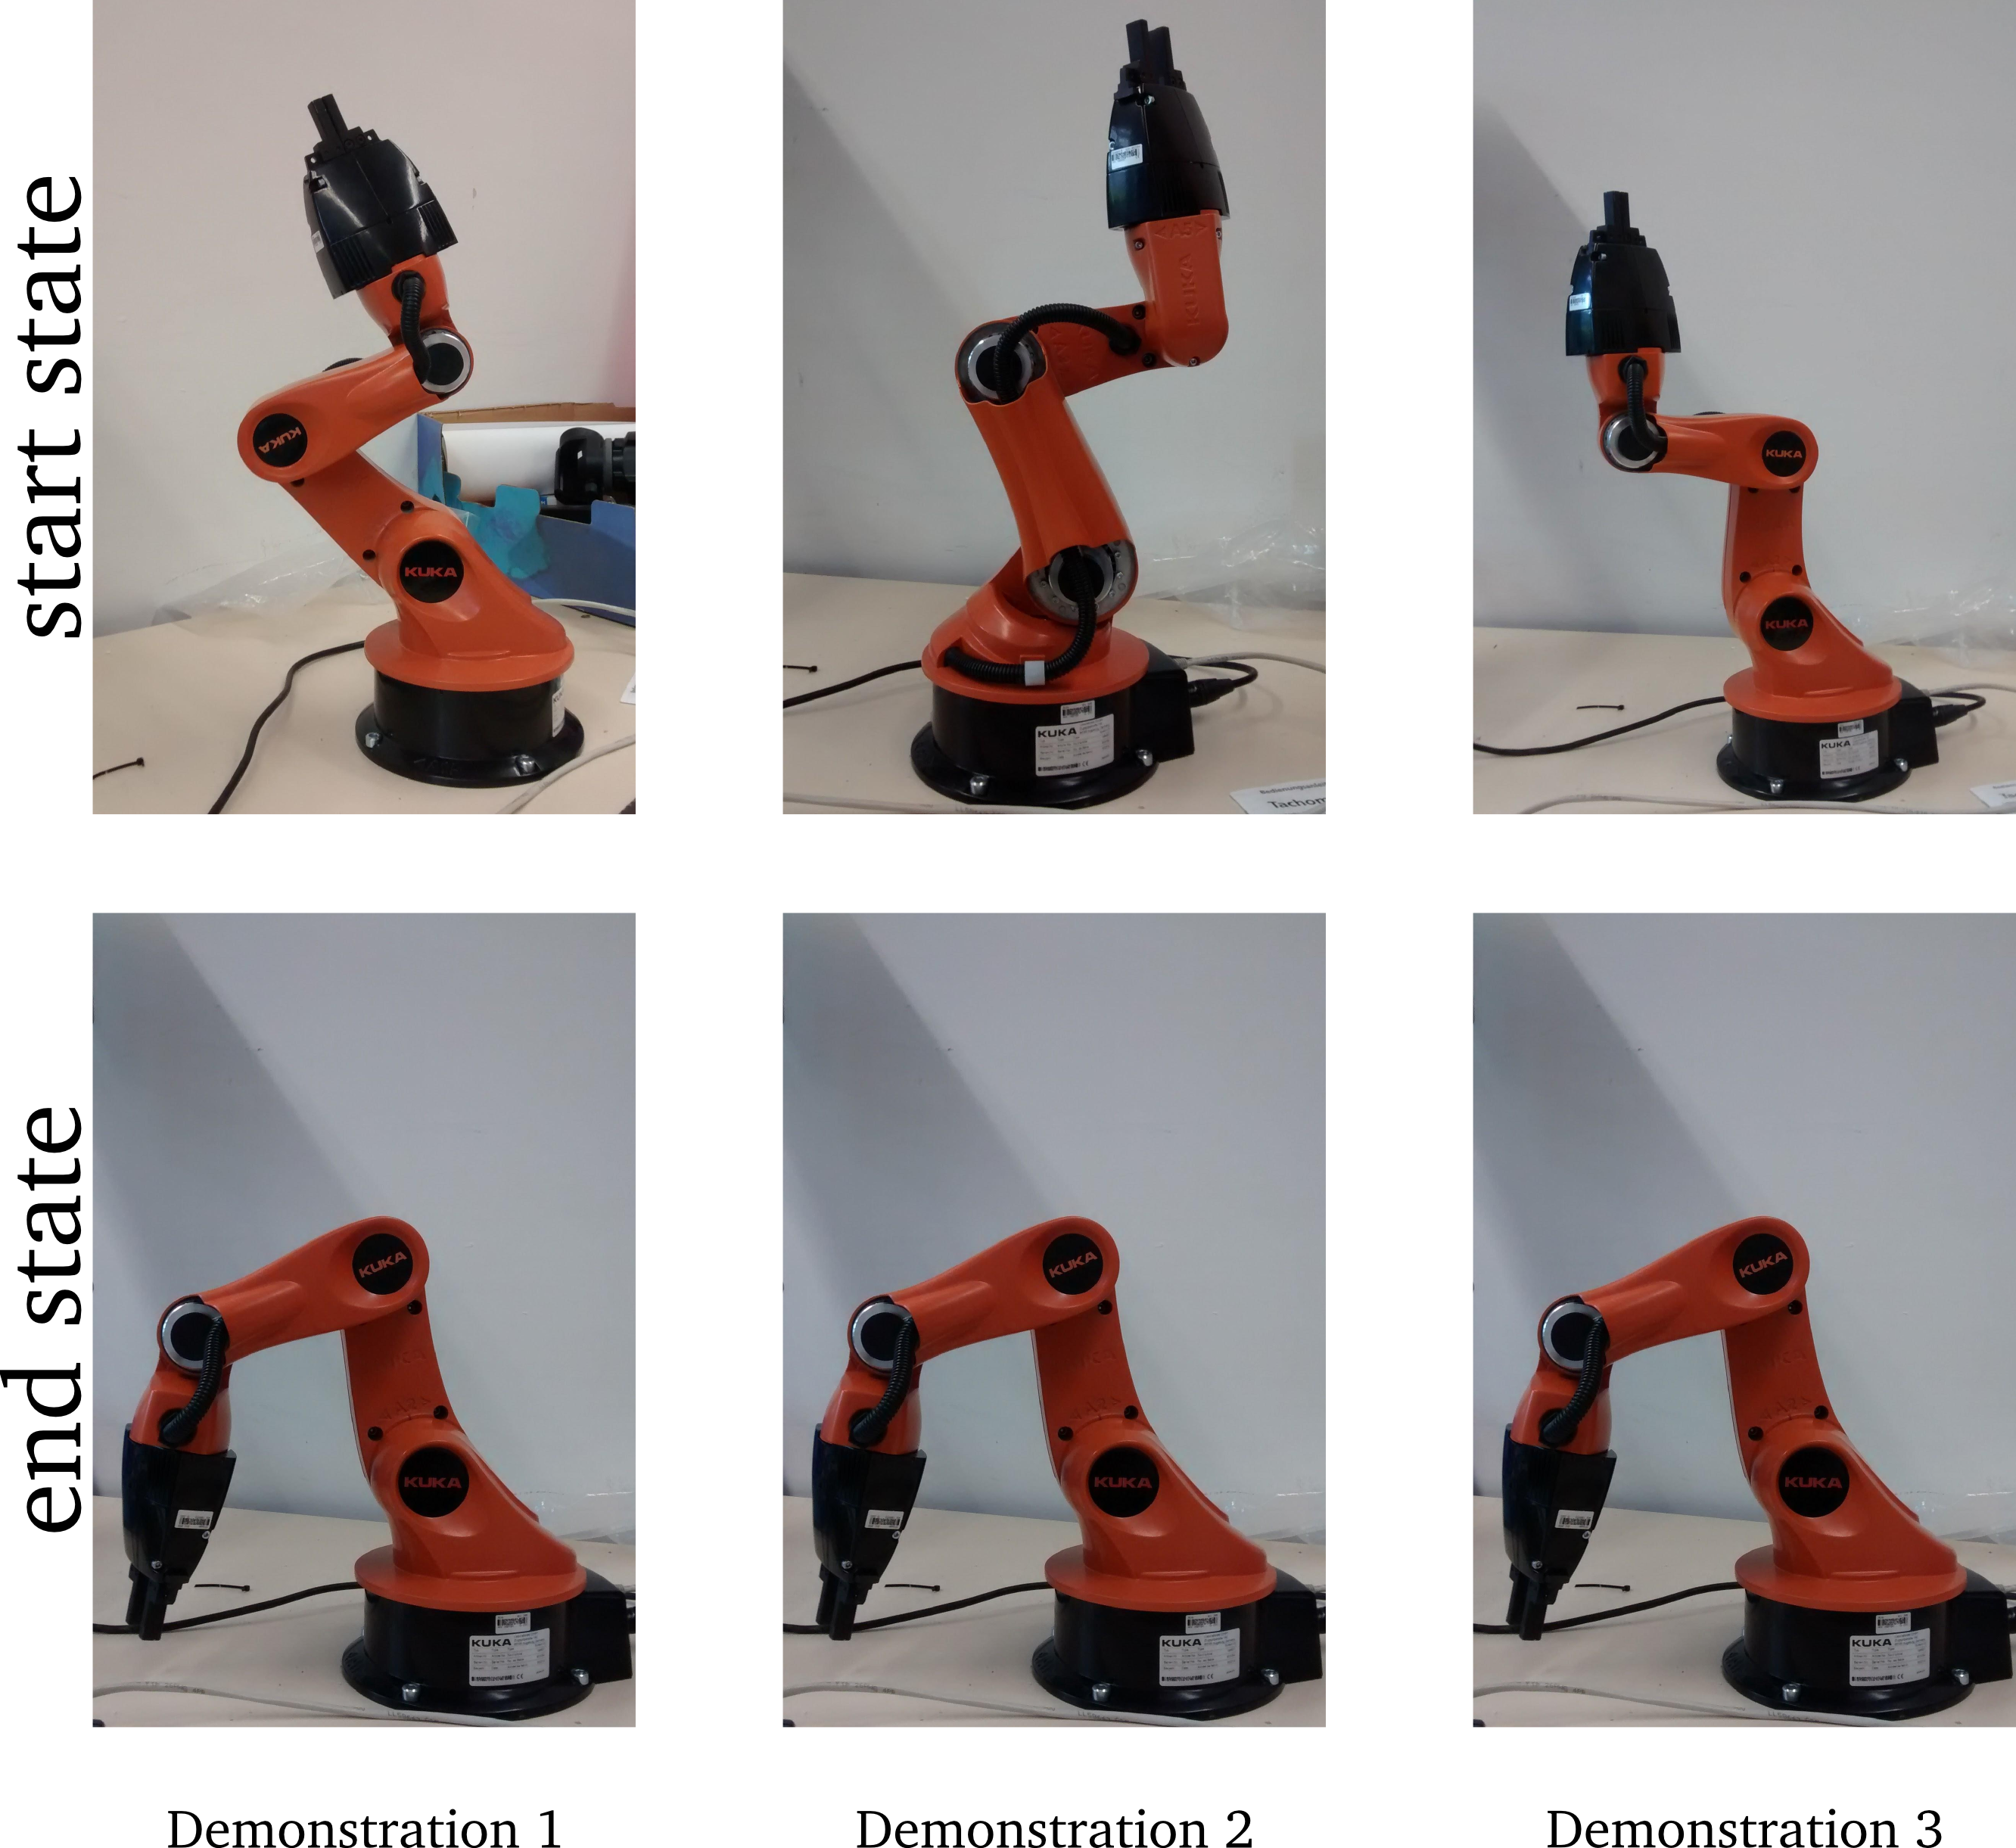
\includegraphics[scale=0.6]{images/arm_absolute_exp.png}
\caption[Demonstrations to teach the robot to move arm to an absolute location ]
{Demonstrations for teaching the robot to \textit{move} arm
to an absolute pose in the workspace. The rows show the recorded start pose and the end pose. The 
columns show the different demonstrations}
\label{arm absolute exp}
\end{figure}

\begin{figure}[htp]
\centering
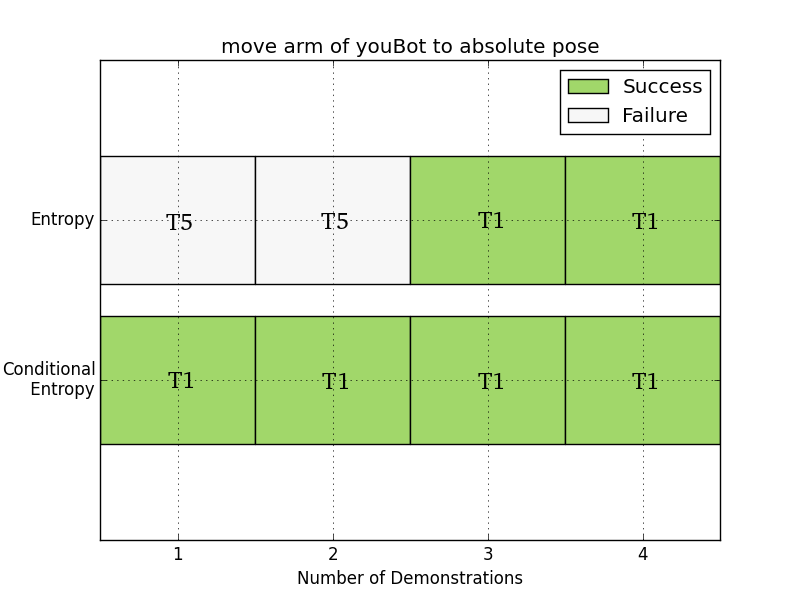
\includegraphics[scale=0.5]{images/arm_absolute_result.png}
\caption[Result : \textit{move} arm absolute pose]{Results of \textit{ move} arm to an absolute pose. The x-axis denotes the 
number of demonstrations used for learning. The y-axis denotes the method used for 
computing relevance.Each
box is marked with the selected template name. Green color denotes the relavant template was successfully recommended}
\label{arm absolute result}
\end{figure}


\FloatBarrier
\subsubsection{\textit{move} arm relative pose to object}
In this experiment the youBot is
taught to \textit{move} arm to a relative pose to an external object.
The experiments consist of recording different start and end poses of the robot arm. 
First the robot arm is moved to any arbitary position and the start pose is recorded then 
the robot arm is moved to the intended final position which needs to be taught and the end 
pose is recorded. The above steps are repeated till all the observations are recorded.


This particular motion primitive can be used as a part of the "precision placement test" task. In these
task the robot has to be place the object precisely inside a cavity. So the robot has to be taught to place
the object relative to placement cavity.
We ran the experiments using different number of demonstrations and using both entropy 
and conditional entropy for measuring relevance. The success of the experiments are 
shown in figure \ref{arm relative results}. 
The template describing the relative distance between the tooltip and the object  was recommended as the most
relevant template from the demonstrations.
\begin{figure}[htp]
\centering
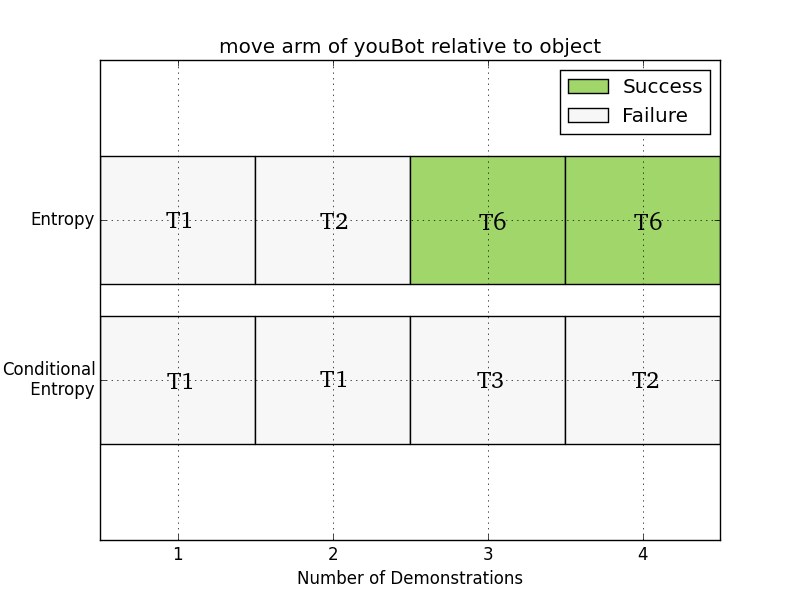
\includegraphics[scale=0.5]{images/arm_relative_result.png}
\caption[Result : \textit{move} arm relative pose to object]{Results of \textit{ move} arm to an relative pose. The x-axis denotes the 
number of demonstrations used for learning. The y-axis denotes the method used for 
computing relevance.Each
box is marked with the selected template name. Green color denotes the relavant template was successfully recommended}
\label{arm relative results}
\end{figure}

\FloatBarrier
\subsubsection{\acrlong{ndcg} based evaluation}
The following section has the evalutaion based on the \acrshort{ndcg}@1 
and \acrshort{ndcg}@2 metrics.
For evalutation the templates in the knowledge base was labeled on a 3 point
likert scale.
We ran the algorithm using entropy as out relevance function.

Figure \ref{ndcg 1} shows the \acrshort{ndcg}@1 plots for different number of 
demonstrations. Its clear that with 3 demonstrations the algorithm is able to
predict the expected template in all the experiments.

Figure \ref{ndcg 3} shows the \acrshort{ndcg}@3 plots for different number of 
demonstrations. We can observe that with increasing number of demonstrations the
quality of the recommendations are improving. With 3 demonstrations the 
quality of the recommendations is well above 60\% for all the experiments.

\begin{figure}[htp]
\centering
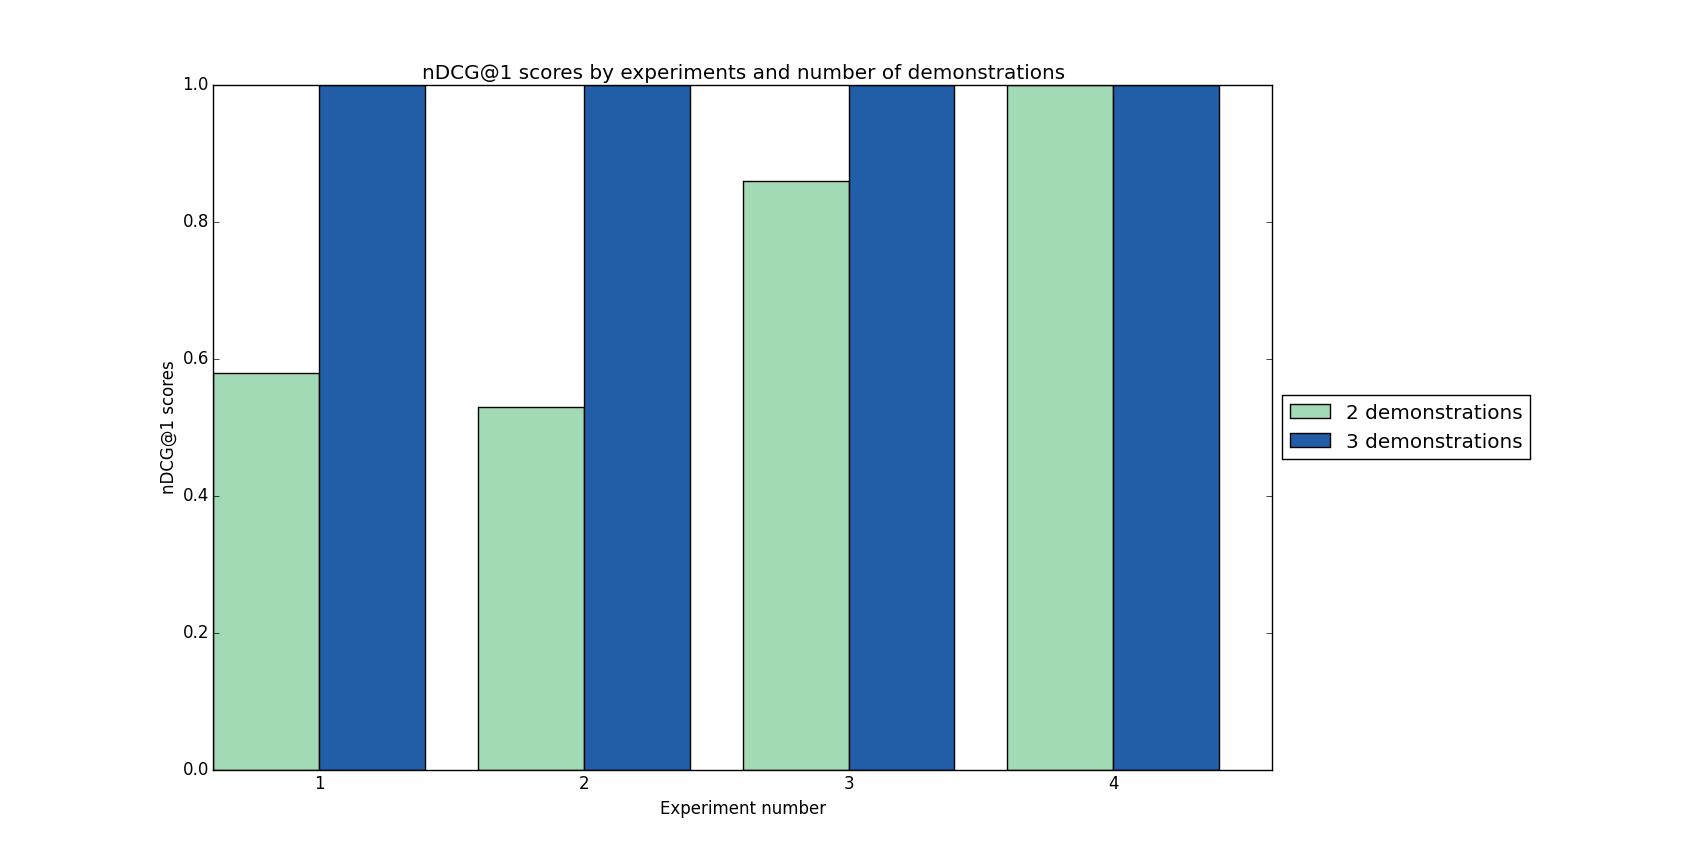
\includegraphics[scale=0.4]{images/nDCG@1.png}
\caption[nDCG@1 score based comparison]{nDCG@1 values for the experiments conducted.
The y-axis is the nDCG@1 score. The x-axis consist of groups of 2 bars arranged
as experiments conducted. Each bar in the experiment corresponds to the number
of demonstration used to make the recommendations. }
\label{ndcg 1}
\end{figure}

\begin{figure}[htp]
\centering
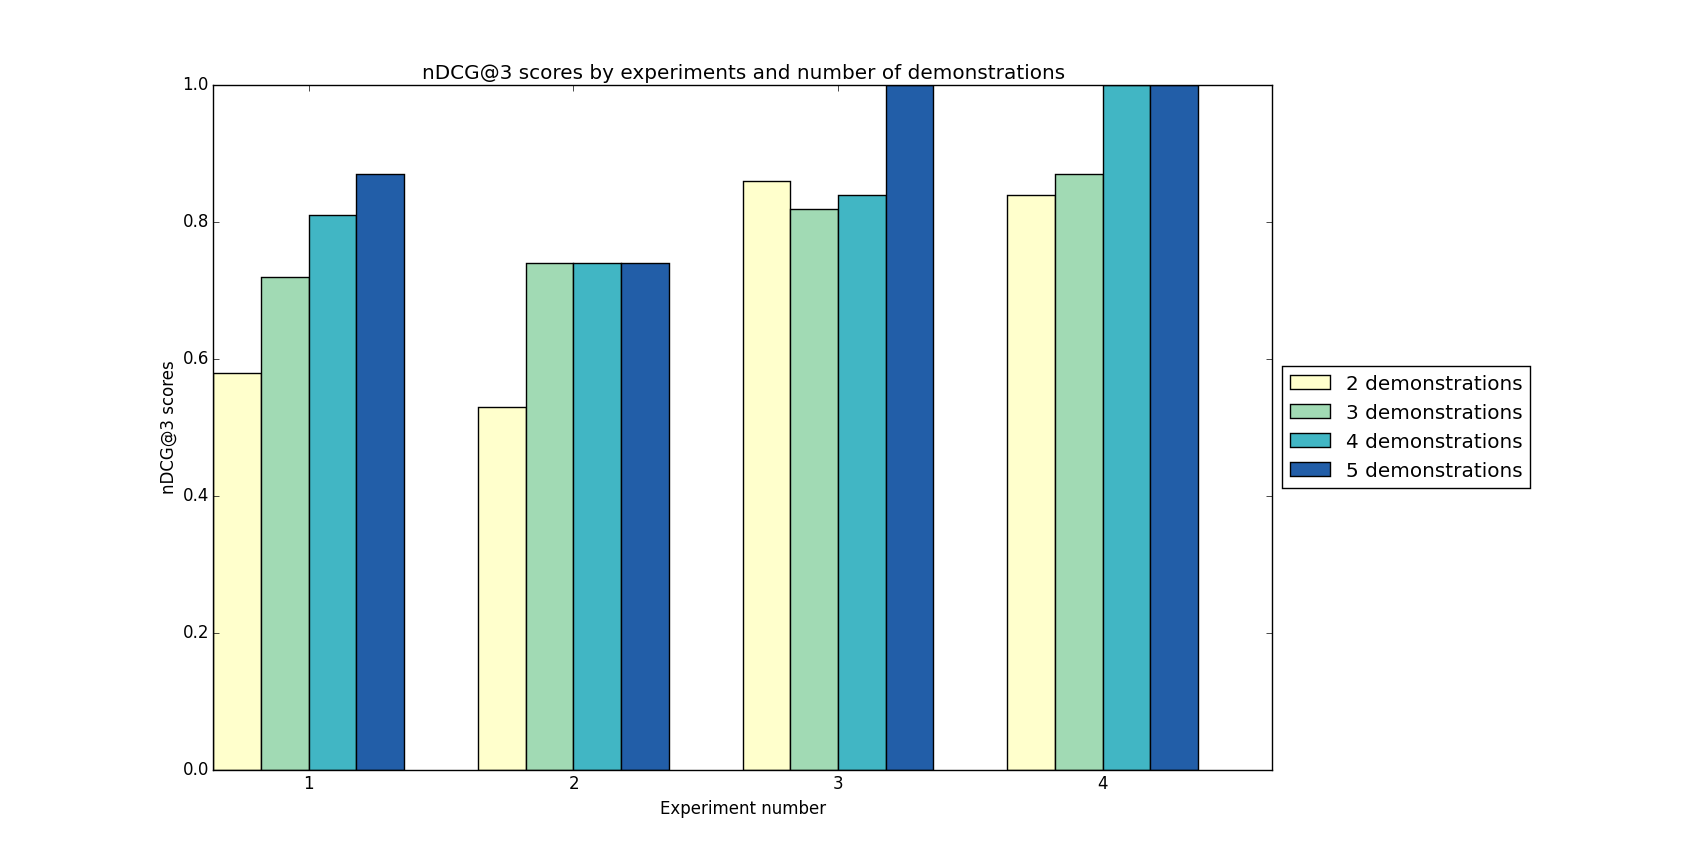
\includegraphics[scale=0.4]{images/nDCG@3.png}
\caption[nDCG@3 score based comparison]{nDCG@3 values for the experiments conducted.
The y-axis is the nDCG@3 score. The x-axis consist of groups of 4 bars arranged
in the sequntial order of the  experiments conducted. Each bar in the experiment corresponds to the number
of demonstration used to make the recommendations. }
\label{ndcg 3}
\end{figure}
\FloatBarrier
\subsection{Discussions}
The proposed approach recommends the relevant features with higher probability.
It has been observed that using entropy based likehood measuring method we could
achieve a success rate of 100\% using just 3 demonstrations.
The higher success rate ensure that the entropy based method is a reliable way to
determine the relevant features.
While using the conditional entropy based relevance measuring method we could 
only achieve a success rate of 62.8\%. 
The lower success rate means that conditional entropy cannot be used for recommending 
the relevant features.


\newpage
\section{Summary} 
In this work we presented relevant feature selection based on
a knowledge base recommendation. The proposed approach was an 
extension to the framework proposed by \cite{abdo_inferring_2014}.

We have proposed a possible framework for representing a motion primitive 
in a skill based framework by \cite{pedersen_robot_2015} . 


Our results show that robot trained using our recommendations not only learns
the goal on demonstrated Motion primitives, but also generalizes well to do
Motion Primitives from initial configurations not demonstrated before.

Our application scenarios of learning goal from demonstrations goes beyond the
application scenarios that previous work has considered.

\newpage
\section{Limitations of work}

This section lists some of the major limitations of the approach.
\begin{itemize}
    \item \textit{Poor quality of demonstration} \\
As \acrshort{lfd} systems are totally dependent on the demonstration of the data, its 
quality greatly reflects on the results. Poor quality of demonstration will lead to 
very poor results. For example in our approach its very much necessary that there has 
to be significant ddifference in the features which are not to be learned. So the 
demonstrations has to vary for all the features not being learned. So great care has to 
be taken by the user to teach a correct set of demonstration.

    \item \textit{Lack of element for feedback} \\
The proposed approach there is not provisions for providing feedback to the robot after
the learning. This is major limitation in terms of learning. Feedback are a good way for 
the robot to generalize on new situations.

    \item \textit{Lack of continuous learning} \\
The proposed approach the learning is done in a single shot. There is no provision for 
feedback and continuos learning. A scalable approach would be if there are provisions 
for the robot to continuos learn while executing. Such provisions will ensure that the 
robot is continuously learning and improving its decision making.


\newpage

\end{itemize}
\section{Future Work}
This section proposes areas that can be improved or extended for future works 
in the field

\begin{itemize}
    \item \textit{Learning "When to imitate" } \\
        The current work only focussed on the "what to imitate" part for identifying
the relevant aspects of the demonstrations. "When to imitate" is a section of 
\acrshort{lfd} to determine when the demonstrated action should be executed.
The proposed approach can be used to identifying the start conditions (pre-condition)
by identifying the relevant aspects in the start values of the demonstrations.

    \item \textit{Better evaluation strategies} \\
        The current evaluation method is manual and are subject ot faults. Automated
methods for evaluting the results need to be used for better confidence on the results.

    \item \textit{Combining both entropy and conditional entropy } \\
The current results showed that entorpy based relevance performed better while
conditional entorpy didnt perform better for all the cases. But conditional entropy 
performed better  in some cases. This needs to be further investigated why the 
conditional entropy didnt perform better in some experiments and how we can modify 
the approach to use it for getting better results.

    \item \textit{Creating a complete skill based on the proposed motion primitive framework}\\
A motion primitive framework is proposed in this work. The relevant features were also 
learnt. Now the work has to be extended to use the relevant feature and execute a particular
motion primitive successfully. Also a set of motion primitives has to be learnt and 
a complete skill has to be executed.

    \item \textit{Better \acrfull{hmi}} \\
The current methods of recording the demonstrations are not sutiable for outside lab.
Since one of the big benefits of \acrshort{lfd} is that non-experts would be able to 
teach the robot with new skills, its of high importance to work on better more intuitive 
\acrshort{hmi} needs to be developed.

    \item \textit{Learning of the templates on-line} \\
The templates used in the approach is generated manually using experts of manipulation.
But in future these futures has to be learnt on-line. The base templates can be used 
from the off-line process but these needs to be updated online based on the demonstrations.
For example for a motion primitive representing the distance between tool-tip and object template will 
be recommended, also if joint 4 is showing relevance as in all the demonstrations joint 4 
was show in a particular angle, then it should be added on-line to the 
template list.

    \item \textit{Completenes of the approach} \\
The results of the approach shows positive signs of the usefullness of the approach.
But we need to have a critical look at the completeness of the solution i.e. can the
approach be generalized for learning all the motion primitives required for a general 
robot. Works like \cite{bogh_does_2012} have claimed that for all the task in an 
industrial setup, a limited list of skills is sufficient. The completeness of our 
approach needs to be verified.

\end{itemize}




\newpage
\appendix
\section{Use of Motion Primitive in Skill Based Framework}
Similar to the concept that speech consist of syllables , it
has been observed that tasks in industrial environments can be broken down into
smaller elements which are called as skills. 
The skills in turn can be decomposed of smaller atomic movements called as Motion Primitives.
A  three layer Framework was introduced by \cite{pedersen_robot_2015} and is illustrated in figure 1.


\begin{figure}[htp]
\centering
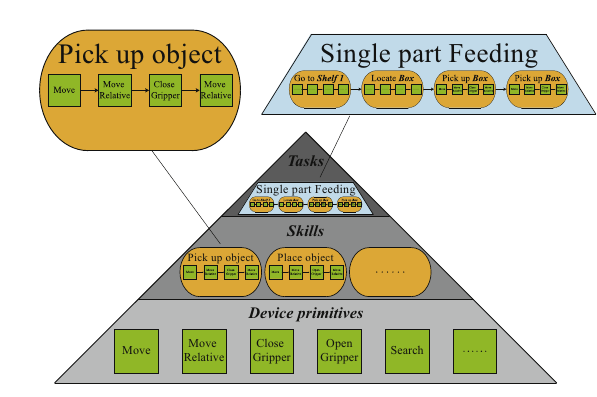
\includegraphics[scale=0.5]{images/skill_framework.png}
\caption[Skill based framework]{Three layers of primitives, skills and tasks. The components in each layer is essentially a combination of lower layer. \cite{pedersen_robot_2015}}
\label{}
\end{figure}

The Three layers can be broken down as follows :
\begin{itemize}
    \item Motion Primitives
    \item Robotics Skills
    \item High Level Tasks
\end{itemize}

\subsection{Motion Primitives}
The lowest layer is the called the motion primitives

% subsection  (end)
\subsection{Robotics Skills}
Robotic skills form the base of the skill based Framework.
Robotic skills are object-centred robot abilities, which can be easily parametrized.
  
% subsection  (end)

\subsection{High level Tasks}
The Higher level description of a task to be done. Ususally in this layer planners like STRIPs or PDDL 
are used to choose which robotic skills has to be executed.

% section  (end)

\section{Knowledge base generator}
\label{knowledge base generator}
\begin{figure}[htp]
\centering
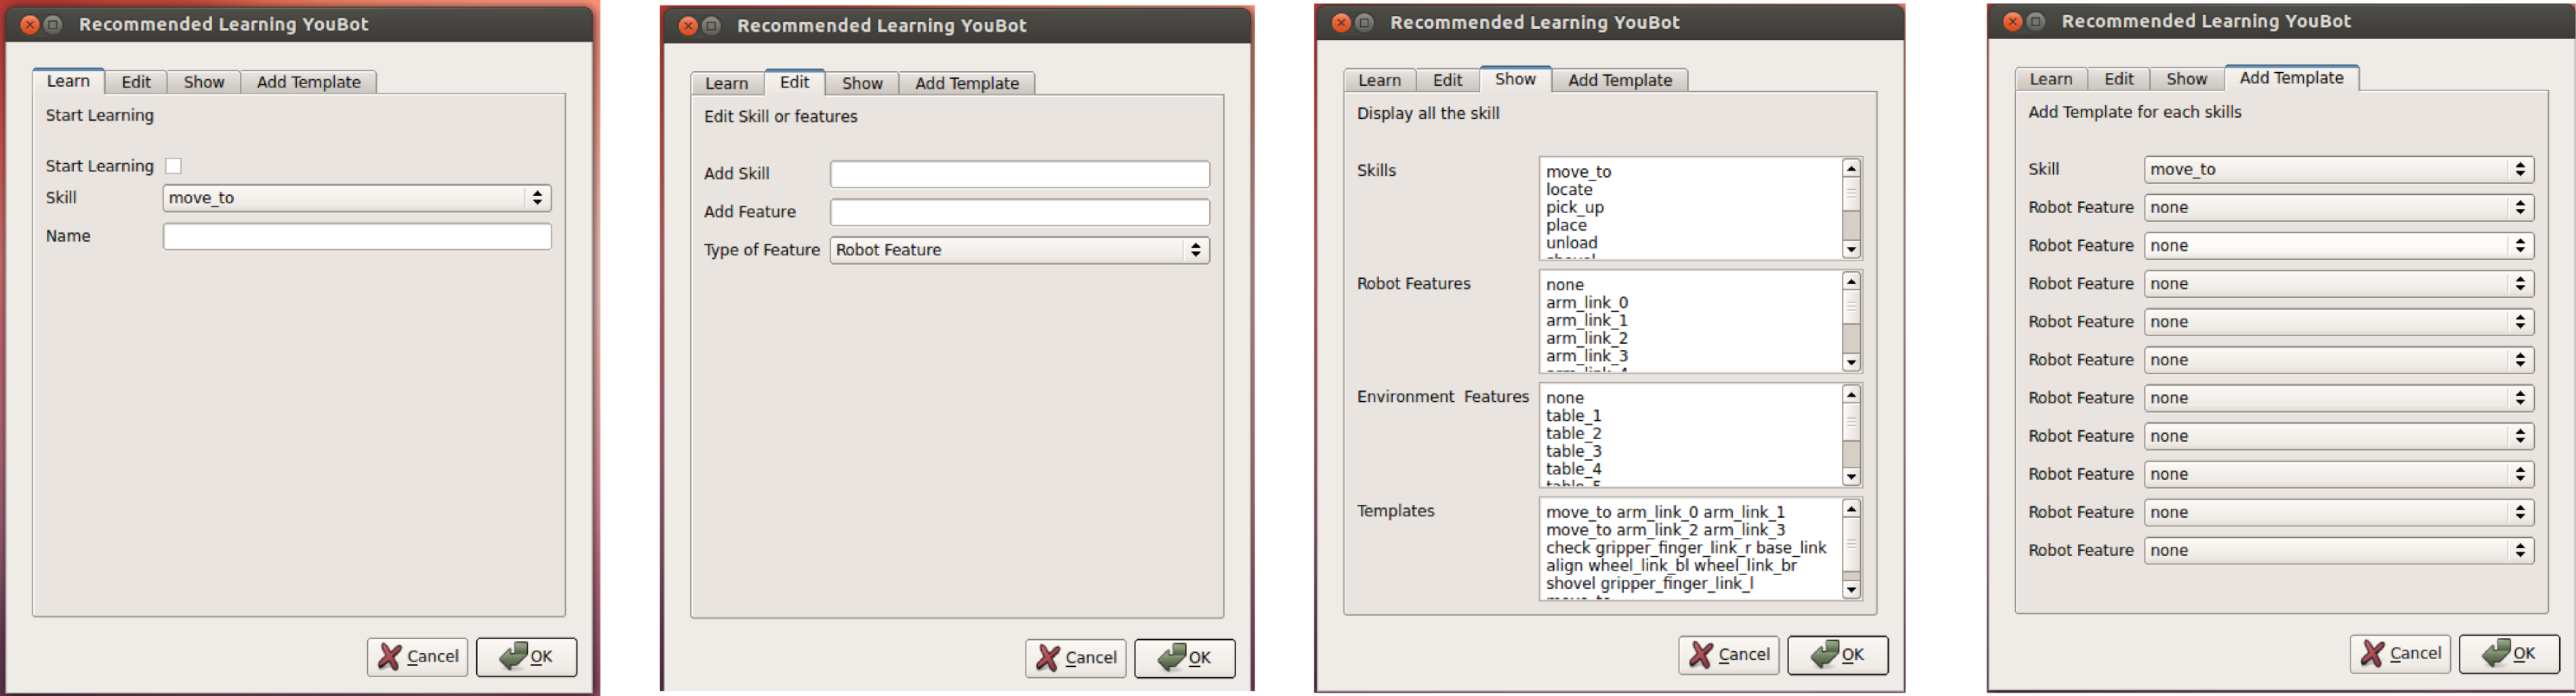
\includegraphics[scale=0.5]{images/tool/tool.png}
\caption[Tool for generating knowledge base]{Tool for generating knowledge base. 1) window for learning a new skill
2) window for editing skill or features 3) Display all features, skills and
templates 4) adding new templates}
\label{}
\end{figure}

On of the limitations of the current efforts in \acrshort{lfd} is adding new features for
new task \cite {argall_survey_2009}. Due to the intuitive nature of
demonstration, \acrshort{lfd} algorithms have the potential to make robot programming
accessible for everyday users who have no programming experience and want to
customize robot behaviours. The use of current approaches by the researchers
, however, is likely to lead to situations in which users attempt to
teach the robot tasks that cannot be learned simply due to the lack of features
describing some aspect of the task.

The solution to such an attempt would be have good tool where the user on 
identification of new features can add new features to the system on which 
the robot can learn.

Also the template creation is an actively changing scenario with various permutations
and combinations possible. The above mentioned tool can be used for rapid 
generation and modification of the templates.


\newpage
\section{Use of Recommender system in robotics}
We started our work based on the notion of using Recommender system in the 
field of robotics. We could partially use the notion of recommender system 
in our work. In the time period of the research various other fields where
the recommender system could be used were identified.
This section list some of the fields of robotics in which technology of 
recommender system fits appropriately.

\subsection{Preferences of users in Task Planing}
With the rise of service robotics in home environments, 
personalized task planning is emerging as a new field of interest.
The robots has to learn the user preferences based on its experience 
with the user and able to modify its decisions regularly.
A common example would be suppose if a user asks the robot for a cup of 
tea, the robot has to make a decision on which cup would be an appropriate 
choice for the user. This choice of the user can be learnt using 
recommender systems.
Works by \cite{abdo_learning_2013} and \cite{abdo_robot_2015} have already 
made progress in this field by using crowd sourcing data.

\subsection{Kernel Recommendation in learning algorithms}
"Firstly, linearity is rather special, and outside quantum mechanics no
model of a real system is truly linear. Secondly, detecting linear
relations has been the focus of much research in statistics and machine
learning for decades and the resulting algorithms are well understood, well
developed and efficient. Naturally, one wants the best of both worlds. So, if a
problem is non-linear, instead of trying to fit a non-linear model, one can map
the problem from the input space to a new (higher-dimensional) space (called
the feature space) by doing a non-linear transformation using suitably chosen
basis functions and then use a linear model in the feature space. This is known
as the 'kernel trick'. The linear model in the feature space corresponds to a
non-linear model in the input space. This approach can be used in both
classification and regression problems. The choice of kernel function is
crucial for the success of all kernel algorithms because the kernel constitutes
prior knowledge that is available about a task. Accordingly, there is no free
lunch (see No Free Lunch Theorems) in kernel choice."
\footnote{\url{http://www.svms.org/kernels/}}

Collaborative based recommender system can be used to determine the kernel 
for learning algorithms. This problem is similar to the n-bandit problem where
the user has to decide on which kernel to keep the bet.

\cite{matikainen_multi-armed_2013} tried to solve the n-bandit problem to
determine which state machine gives better coverage of the floor.
Similar attempts can be made in learning the kernel .

\subsection{Motion Path Planning algorithms }
\acrfull{ompl} has implemented the following planners \url{http://ompl.kavrakilab.org/planners.html}
The selection of the planner for a particular tasks is active scientific 
problem.
If you use the \acrshort{ompl} control , then \acrshort{ompl} will automatically select an
appropriate planner (unless you have explicitly specified one).
If the state
space has a default projection (which is going to be the case if you use any of
the built-in state spaces), then it will use \acrfull{kpiece}. This planner has been
shown to work well consistently across many real-world motion planning
problems, which is why it is the default choice.
In case the state space has no
default projection, \acrfull{rrt} will be used. 
Can we recommend which planner to use in which situation based on previous 
knowledge of the planner in similar situations.
Content based recommender system can be used in such situations to determine 
which planner will be suitable in current situation.

\subsection{Learning trajectory preference of users}
\cite{jain_learning_2013} have worked on learning the trajectory preferences 
of users by on-line learning their feedbacks.
Similar approach can be used as a recommender system to learn 
the user preference of a trajectory for doing a particular tasks.

\newpage
\section{Softwares and tools}

A software implementation and number of tools have been included in the attached
$CD\-ROM$. The tools and the software developed as part of the project.
Below is a brief description of the packages

\begin{itemize}

    \item \textbf{Recommender Learning} \\
        Python based implementation of the learning approach. The class has to be 
        invoked with the folder containing the JSON file of the demonstrations.
        The JSON file is read and learning is made on base of the demonstrations.
        It also reads the knowledge base and creates the set of templates.
        It implements the approach mentioned in section \ref{sec:Learning motion primitive}.
        Available online : \url{https://github.com/deebuls/RecommenderSystemInRobotics/tree/master/code/recommended\_learning}

    \item \textbf{mir\_teleop\_record} \\
        ROS node for teleoperation of the youbot arm and the base. The node was 
        an extension of the work of b-it bots team \url{https://github.com/mas-group/robocup-at-work/tree/brazil-2014/mas\_common\_robotics/mcr\_tools/mcr\_teleop}.
        The node was modified to record the features and to create a JSON file with the readings.
        Available online : \url {https://github.com/deebuls/RecommenderSystemInRobotics/tree/master/code/mir\_teleop\_record }

    \item \textbf{Data accumulator} \\
        The python script for accumulating all the recorded json file and creating
        a consolidated JSON file of the demonstration.
        Available online : \url{https://github.com/deebuls/RecommenderSystemInRobotics/tree/master/code/tools }

    \item \textbf{Knowledge base creator} \\
        An interactive online tool for creating of the knowledge base.
        Menu driven GUI for active interaction with the user and easy to use
        template creation for the knowledge base.
        Available online : \url{ https://github.com/deebuls/RecommenderSystemInRobotics/tree/master/code/knowledge\_base\_creator}

\end{itemize}


\newpage
% create bibtex document
\bibliographystyle{apalike} % mit Buchstaben
%\bibliographystyle{plain} % normal
%\bibliographystyle{unsrt} % in reinfolge des Textes
% \bibliographystyle{abbrv} % wie plan , nur abgekürtz

\bibliography{BibTex}
%\bibliography{robotics_skill}



%\bibliography{BibTex.bib}{}
%\bibliographystyle{plain}
\end{document}


